% ============================================================
%  ROZDZIAŁ: Część badawcza
% ============================================================

\newpage
\graphicspath{{data/5 - badania/wykresy/}}
\section{Część badawcza: analiza porównawcza i optymalizacja SLM na urządzeniu brzegowym}
\label{sec:modele}

Część badawcza stanowi zasadniczy punkt niniejszej pracy magisterskiej.
Jej celem było empiryczne sprawdzenie, na ile mały model językowy może
działać użytecznie na urządzeniu brzegowym o~bardzo ograniczonych zasobach.
Raspberry~Pi~5 z~8~GB pamięci RAM, bez dedykowanego GPU, wymusza kompromisy
między jakością odpowiedzi, opóźnieniem oraz stabilnością inferencji; bez
systematycznych pomiarów trudno byłoby uzasadnić wybór modelu, kwantyzacji
czy konfiguracji generacji w~takim środowisku.

W~rozdziale zbadano m.in.\ wpływ hiperparametrów Ollamy, wariantów kwantyzacji
GGUF oraz warunków pomiaru (w~tym stanów \emph{cold} i~\emph{warm cache})
na metryki jakościowe i~wydajnościowe lokalnego SLM. Choć eksperymenty
przeprowadzono w~kontekście asystenta głosowego systemu Wilga~MiLL, uzyskane
wnioski mają charakter ogólniejszy: dotyczą uruchamiania małych modeli
językowych na typowym sprzęcie IoT i~mogą być wykorzystane także w~innych
aplikacjach brzegowych o~podobnych ograniczeniach pamięci i~mocy obliczeniowej.

% ============================================================
\subsection{Architektura i metodologia systemu benchmarkowego}
\label{subsec:metodologia}
% ============================================================

\subsubsection{Komponenty systemu testowego}

Założeniem dla budowy systemu testowego nie było uruchamianie pełnego produkcyjnego pipeline'u aplikacji Wilga, lecz
stworzenie wycinka systemy, który pozwoli poddać testom modele SLM na urządzeniu brzegowym. Architektura systemu pomiarowego składa
się z~dwóch bloków: serwera orkiestrującego (MacBook) oraz
platformy brzegowej (Raspberry~Pi~5), przedstawionych na
rysunku~\ref{fig:testy_arch}.

Po stronie serwera pracuje skrypt \texttt{tester.py}, który pełni rolę orchestratora. Dla
każdego przypadku z~\texttt{golden.jsonl} pobiera \emph{system\_prompt},
łączy go z~pytaniem użytkownika i~wysyła żądanie HTTP do Ollamy uruchomionej
na Raspberry~Pi. Po stronie serwera mierzone są parametry czasowe: TTFT(time to first token) oraz E2E(end to end). Po otrzymaniu odpowiedzi modelu
orkiestrator przekazuje ją do modelu zewnętrznego oceniającego jakość odpowiedzi. Ponownie korzystając z OpenRouter podłączono się do modelu Claude, tym razem był to Haiku 3.5. Zastosowano mniejszy, tańszy model, gdyż benchmark wymagał wysyłania wielu żądań, a koszty największych modeli są wygórowane. Haiku zwracał pięć metryk jakościowych, opisanych w~tabeli~\ref{tab:haiku_metryki}.

Prompt przekazywany do Haiku składał się z~czterech elementów wejściowych:
\begin{equation}
  \label{eq:haiku_prompt}
  \mathrm{prompt}_{\mathrm{Haiku}}
  =
  \{\mathrm{system\_prompt}\}
  +
  \{\mathrm{question}\}
  +
  \{\mathrm{golden\_answer}\}
  +
  \{\mathrm{model\_answer}\},
\end{equation}
\noindent
gdzie \emph{system\_prompt} to kontekst stanu domu zbudowany wcześniej
z rzeczywistych wierszy danych sensorowych, \emph{question} to pytanie użytkownika, \emph{golden\_answer}
odpowiedź wzorcowa, natomiast \emph{model\_answer} to odpowiedź badanego SLM.
W~prompcie wskazano ponadto, że kontekst sensorowy jest jedynym źródłem
prawdy, a~wynik musi zostać zwrócić jako JSON z~pięcioma metrykami. Flaga halucynacji miała być ustawiana tylko wtedy, gdy model
podaje konkretne fakty spoza kontekstu. Temperaturę ewaluacji ustawiono
na zero, żeby oceny były możliwie powtarzalne. Otrzymana odpowiedź była przetwarzna oraz odrzucana jeśli format nie odpowiadał żądanemu JSON. Wymuszenie pozostaje jednak miękkie, w przypadku dalszej ewaluacji testów za istotne uznano zastosowanie mechanizmów takich jak \href{https://ai.pydantic.dev/output/}{Pydantic AI} czy \href{https://docs.langchain.com/oss/python/langchain/structured-output}{LangChain} pozwalających deterministycznie definiować format odpowiedzi modeli językowych.

Na urządzeniu brzegowym Raspberry Pi 5 działa serwer Ollamy, który dzięki funkcji API pozwala na łatwe odpytywanie wielu modeli zainstalowanych na urządzeniu. Eównolegle działał również mikroserwer \texttt{metrics\_server.py}, jego wprowadzenie było konieczne aby mierzyć temperaturę CPU, zużycie RAM oraz flagę dławienia (throttling flag, przegrzanie procesora).

\begin{figure}[H]
  \centering
  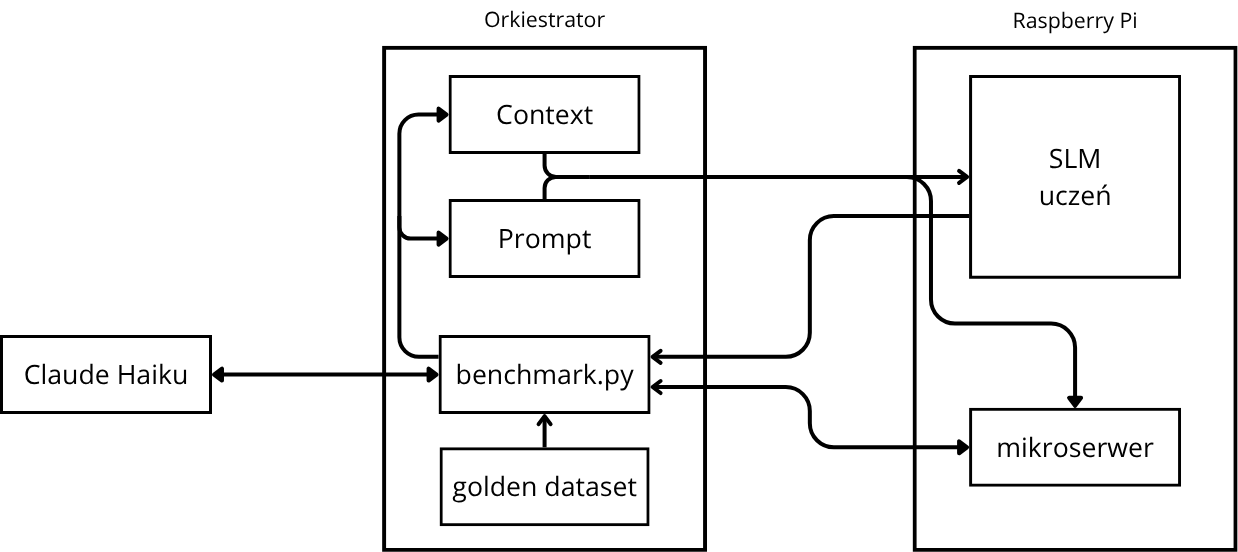
\includegraphics[width=0.85\textwidth]{src/img/testy-schemat.png}
  \caption{Schemat systemu benchmarkowego. Serwer (MacBook~M4) pełni rolę
           orchestratora i~hosta ewaluatora; Raspberry~Pi~5 jest platformą
           inferencji.}
  \label{fig:testy_arch}
\end{figure}

\subsubsection{Zbiór danych testowych}


Pracę nad częścią badawczą rozpoczęto od zbiory zawierającego pytania oraz modelowe odpowiedzi. Jest nim plik \texttt{golden.jsonl}: stały zbiór 20~przypadków testowych. Każdy rekord zawiera identyfikator
przypadku, jego kategorię, tekstowy \emph{system\_prompt} zbudowany z~realnego
wiersza danych sensorowych, pytanie użytkownika oraz
wzorcową odpowiedź \emph{golden\_answer}. Zbiór wygenerowano jednorazowo przy użyciu modelu Claude Sonnet~4.6. Wybór modelu znacznie większego i~bardziej zaawansowanego od lokalnie uruchamianych modeli (omawianych w pracy) pozwolił zapewnić wysoką jakość odpowiedzi referencyjnych. Do integracji i~wywołania modelu wykorzystano API platformy \href{https://openrouter.ai}{OpenRouter}, będącej wygodnym agregatorem modeli językowych od wielu dostawców.

Rozkład kategorii przypadków przedstawiono w~tabeli~\ref{tab:golden_kategorie}.

\begin{table}[H]
  \centering
  \caption{Kategorie przypadków w~złotym zbiorze testowym (20~przypadków).}
  \label{tab:golden_kategorie}
  \begin{tabular}{lrl}
    \hline
    Kategoria & Liczba & Co testuje \\
    \hline
    \texttt{factual\_status}   & 8 & Poprawne odczytanie stanu z~kontekstu \\
    \texttt{missing\_data}     & 4 & Przyznanie braku danych zamiast zgadywania \\
    \texttt{conflicting\_data} & 3 & Wykrycie sprzeczności w~danych \\
    \texttt{stale\_data}       & 2 & Sygnalizacja nieaktualności odczytu \\
    \texttt{paraphrase}        & 3 & Spójność odpowiedzi na te same pytania \\
    \hline
    \textbf{Razem}             & \textbf{20} & \\
    \hline
  \end{tabular}
\end{table}

Kategorie \texttt{missing\_data} i~\texttt{stale\_data} uznano za najbardziej wymagające,
ponieważ są podatne na halucynacje, która jak zaznaczono w analizie literatury \ref{sec:analiza_literatury} jest krytycznym czynnikiem w ocenie jakości odpowiedzi modeli językowych.

\subsubsection{Metryki oceny i wzór composite score}
\label{subsec:metryki}

\begin{table}[H]
  \centering
  \caption{Metryki oceny stosowane w~benchmarku (trzy grupy).}
  \label{tab:haiku_metryki}
  \begin{tabular}{cllp{5.6cm}}
    \hline
    Grupa & Metryka & Zakres & Znaczenie \\
    \hline
    1 & TTFT & ms & Czas do pierwszego tokenu \\
    1 & E2E & ms & Czas do ostatniego tokenu \\
    1 & \emph{generation\_ms} & ms & $\mathrm{E2E}-\mathrm{TTFT}$ \\
    1 & RAM & MB & Zużycie pamięci na Raspberry~Pi \\
    1 & temperatura CPU & $^\circ$C & Temperatura procesora z~mikroserwera \\
    1 & flaga dławienia & binarna & Przegrzanie / throttling procesora \\
    \hline
    2 & \texttt{faithfulness} & $[0,1]$ & Czy każde twierdzenie faktyczne wynika z~kontekstu sensorowego \\
    2 & \texttt{answer\_relevancy} & $[0,1]$ & Czy odpowiedź adresuje zadane pytanie \\
    2 & \texttt{conciseness} & $[0,1]$ & Czy odpowiedź jest zwięzła, bez zbędnych informacji \\
    2 & \texttt{hallucination\_flag} & binarna & \texttt{true}, gdy odpowiedź zawiera fakty spoza kontekstu; zeruje wynik łączny \\
    \hline
    3 & \texttt{polish\_quality} & $[0,1]$ & Naturalność i~poprawność języka polskiego; rejestrowana, poza \emph{composite score} \\
    \hline
  \end{tabular}
\end{table}

Metryki z~tabeli~\ref{tab:haiku_metryki} podzielono na trzy grupy.
Grupa~1 obejmuje metryki wydajnościowe mierzone deterministycznie przez urządzenie brzegowe.
Grupa~2 to metryki jakościowe zwracane przez LLM-oceniający (Haiku~3.5).
Grupa~3 obejmuje \emph{polish\_quality} został dodany w celu przyszłych ewaluacji jakościowych odpowiedzi.

Metryki z grupy drugiej składają się na \emph{composite score}. W oparciu o literaturę oraz standardy \cite{Es2024Ragas,ConCISE2025,DefAn2024} przyjęto go jako sposób matematycznego wyznaczania jakości odpowiedzi porównywanych modeli. Konieczne 
do wyznaczenia composite score było przyjęcie wag dla każdej z metryk. Wzór przedstawiony w równaniu \ref{eq:composite_score}.

\begin{equation}
  \label{eq:composite_score}
  \mathrm{score} =
  \begin{cases}
    0{,}0 & \text{gdy } \mathrm{hallucination\_flag} = \mathrm{true} \\[6pt]
    0{,}40 \cdot f + 0{,}30 \cdot r + 0{,}20 \cdot c + \ell & \text{w~przeciwnym razie}
  \end{cases}
\end{equation}
\noindent
gdzie $f$, $r$, $c$ to odpowiednio \emph{faithfulness}, \emph{answer\_relevancy}
i~\emph{conciseness}, a~$\ell = 0{,}05 \cdot (1 - \min(\mathrm{e2e\_ms}/90\,000,\, 1))
+ 0{,}05 \cdot (1 - \min(\mathrm{ttft\_ms}/45\,000,\, 1))$.

W prezenotwanym rozwiązaniu\emph{faithfulness} ma najwyższą wagę, ponieważ odpowiedź trzymająca się faktów jest niezwykle istotna w konktekście tej pracy- asystenta głoswoego. Składniki opóźnienia (E2E
i~TTFT, łącznie 0{,}10) zostały rozdzielone, ponieważ moduł TTS może rozpocząć
syntezę mowy przed zakończeniem generacji tokenów co powoduje wrażenie bardziej płynnej interakcji. 

\subsubsection{Dostrajanie parametrów pracy modelu}

Optymalizację hiperparametrów inferencji modelu przeprowadzono z wykorzystaniem biblioteki Optuna
wykorzystującej metodę TPE (\emph{Tree-structured Parzen Estimator}). Przeszukiwana
przestrzeń współczynnik pracy modelu przedstawiono w~tabeli~\ref{tab:optuna_hparams}.

\begin{table}[H]
  \centering
  \caption{Przestrzeń hiperparametrów przeszukiwana przez Optunę (TPE).}
  \label{tab:optuna_hparams}
  \begin{tabular}{lll}
    \hline
    Parametr & Typ & Zakres \\
    \hline
    \texttt{temperature}    & float       & $[0{,}10,\; 0{,}80]$ \\
    \texttt{num\_ctx}       & categorical & $\{1024,\; 2048,\; 4096\}$ \\
    \texttt{num\_predict}   & int         & $[48,\; 160]$ \\
    \texttt{top\_p}         & float       & $[0{,}80,\; 0{,}99]$ \\
    \texttt{repeat\_penalty}& float       & $[1{,}00,\; 1{,}15]$ \\
    \hline
  \end{tabular}
\end{table}

Pełna siatka parametrów wynosi $8 \times 3 \times 3 \times 5 \times 4
= 1440$ kombinacji $\times$ 20~promptów $= 28\,800$ zapytań. Optuna z~80~trialami (przejściami przez pełny zestaw 20 pytań)
($80 \times 20 = 1600$ ewaluacji LLM-oceniającego) osiąga porównywalne pokrycie
obszarów obiecujących dzięki istocie swojego działania. Nie prowadzono testów Nie na wszystkich modelach przeprowadzano testy tej samej długości.

\subsubsection{Modele kandydujące}

Do badań wybrano sześć modeli klasy SLM, których wielkość zawierała się w przedziale  2--5B parametrów. Kierowano się przede wszystim wielkością modelu oraz postanowiono postawić na znanych dostawców. Tabela~\ref{tab:modele_kandydaci}
przedstawia wybranych kandydatów..

\begin{table}[H]
  \centering
  \caption{Modele kandydujące i~ich udział w~benchmarku Optuny.}
  \label{tab:modele_kandydaci}
  \small
  \begin{tabular}{lllll}
    \hline
    Model & Parametry & GGUF Q4\_K\_M & Producent \\
    \hline
    Llama~3.2~3B  & 3{,}2~mld & ${\sim}$2{,}0~GB & Meta        \\
    Phi-3.5 Mini  & 3{,}8~mld & ${\sim}$2{,}4~GB & Microsoft  \\
    Gemma~2~2B    & 2{,}6~mld & ${\sim}$1{,}7~GB & Google     \\
    Gemma~3~4B    & 4{,}0~mld & ${\sim}$2{,}3~GB & Google     \\
    Qwen~2.5~3B   & 3{,}0~mld & ${\sim}$2{,}0~GB & Alibaba    \\
    Bielik~4.5B   & 4{,}5~mld & ${\sim}$2{,}7~GB & SpeakLeash \\
    \hline
  \end{tabular}
\end{table}


% ============================================================
\subsection{Etap Optuna: chłodzenie, hiperparametry i dominacja halucynacji}
\label{subsec:optuna}
% ============================================================

\subsubsection{Warunek termiczny pomiaru}
\label{subsec:run1}
\label{subsec:run2}

Testy rozpoczęto ze wskazaną wyżej grupą modeli. Bardzo szybko okazało się, że czsy odpowiedzi bardzo często przekraczają górną granicę pomiaru, którą wyznaczono na 60 sekund. Po analizie danych jasna stała się przyczyna.
W~każdym z~500~rekordów procesor pracował
w~trybie throttling (ang. dławienie). Dzięki pomiarom mikroserwera na RPi możliwe było odczytanie temperatury CPU.
Na Raspberry~Pi~5 throttling jest metodą ograniczania częstotliwości taktowania procesora w celu obniżenia temperatury, skutkuje ona znacznym obniżeniem mocy obliczeniowej jednostki. Pierwsze ogaraniczenia aktywowane są przy ~80\,°C, a~twarde
dławienie (\texttt{vcgencmd get\_throttled 0x2}) ok.~85\,°C.

Przy przekroczeniu limitu czasu (60\,s) Ollama zwraca pustą odpowiedź, którą
LLM-judge klasyfikuje jako halucynację (score $= 0$). Odnotowano 169~timeoutów
z~korelacją 100\% względem flagi halucynacji. Dla \texttt{gemma3:4b} 42\%
rekordów kończyło się timeoutem. W~efekcie ranking z~tabeli~\ref{tab:ranking_run1}
był w~zasadzie fałszywy: \texttt{gemma2:2b} zajmował pierwsze miejsce, a~lepszy
semantycznie \texttt{gemma3:4b} spadał na czwarte --- większe modele dłużej
obciążają CPU i~przy braku chłodzenia generują timeouty. Temperatura CPU
utrzymywała się w~zakresie 84{,}0--91{,}7\,°C (mediana 88{,}9\,°C), a~throttling
występował w~100\% przypadków.

\begin{table}[H]
  \centering
  \caption{Ranking modeli bez aktywnego chłodzenia
           ($n=100$ pomiarów na model).}
  \label{tab:ranking_run1}
  \begin{tabular}{clccccc}
    \hline
    \# & Model & Score & Halucynacje & E2E med. [ms] & Mediana temp. [$^\circ$C] & Throttling \\
    \hline
    1 & \texttt{gemma2:2b}  & 0{,}693 & 16\% & 37\,229 & 87{,}8 & 100\% \\
    2 & \texttt{llama3.2:3b}& 0{,}589 & 30\% & 49\,199 & 88{,}4 & 100\% \\
    3 & \texttt{qwen2.5:3b} & 0{,}547 & 37\% & 53\,169 & 88{,}9 & 100\% \\
    4 & \texttt{gemma3:4b}  & 0{,}497 & 42\% & 57\,584 & 89{,}8 & 100\% \\
    5 & \texttt{phi3.5}     & 0{,}024 & 96\% & 60\,000 & 90{,}0 & 100\% \\
    \hline
  \end{tabular}
\end{table}

Jako receptę na problemy termiczne wskazano aktywne chłodzenie procesora. Układ RPi został rozbudowany o radiator producenta wyposażony w wentylator. Po instalacji chłodzenia przeprowadzono test sprawdzający czy przyniosło ono zamierony efekt. Flaga throttlingu nie została oznaczona w żadnym z przypadków testowych (0/500), a~temperatura CPU do 57{,}6--73{,}6\,°C (mediana 65{,}3\,°C). Zmiana wprowadziła też pierwsze niezerowe wyniki \emph{composite\_score} modeli. Wyniki przedstawiono w tabeli \ref{tab:ranking_run2}.

\begin{table}[H]
  \centering
  \caption{Ranking modeli po zastosowaniu aktywnego chłodzenia.}
  \label{tab:ranking_run2}
  \begin{tabular}{clcccc}
    \hline
    \# & Model & Score & Halucynacje & E2E med. [ms] & Throttling \\
    \hline
    1 & \texttt{gemma3:4b}  & 0{,}806 & 4\%  & 31\,742 & 0\% \\
    2 & \texttt{gemma2:2b}  & 0{,}679 & 19\% & 20\,879 & 0\% \\
    3 & \texttt{qwen2.5:3b} & 0{,}667 & 19\% & 29\,713 & 0\% \\
    4 & \texttt{llama3.2:3b}& 0{,}653 & 20\% & 27\,145 & 0\% \\
    5 & \texttt{phi3.5}     & 0{,}380 & 49\% & 52\,363 & 0\% \\
    \hline
  \end{tabular}
\end{table}

Wstępne problemy z~regulacją termiczną CPU uwydatniły
uwydatnić, jak bardzo stabilność temperaturowa warunkuje
ewaluację modeli językowych na urządzeniach klasy Raspberry Pi 5. Nie spotkało się to ze zdziwieniem, gdyż zagadnienie to szeroko opisaywane jest w literaturze \cite{Tummalapalli2026} oraz przez inżynierów w internecie. Aktywne chłodzenie okazało się zapewniać stabilne warunki pracy platformy i~umożliwiło rzetelne przeprowadzenie dalszych badań.

\subsubsection{Dominacja flagi halucynacji}
\label{subsec:hallucination_dominance}

Pełny przebieg Optuny (\texttt{dataset=results-selected-9.05}, 80~triali)
umożliwił analizę źródeł wariancji \emph{composite score}. Regresja
wieloczynnikowa (rysunek~\ref{fig:regression_r2}) wykazała, że sama flaga
halucynacji wyjaśnia $R^2 = 0{,}9922$ wariancji score --- hiperparametry
inferencji wyjaśniają jedynie $R^2 = 0{,}2997$. Model (\texttt{model\_only})
daje $R^2 = 0{,}8201$; dodanie hiperparametrów (\texttt{model\_plus\_hparams})
podnosi $R^2$ do 0{,}8587 ($\Delta R^2 = 0{,}039$). Pełny model osiąga
$R^2 = 0{,}9982$.

\begin{figure}[H]
  \centering
  
\includegraphics[width=0.85\textwidth]{02_score_vs_hallucination_selected.png}
  \caption{Zależność \emph{composite score} od wskaźnika halucynacji
           (\texttt{results-selected-9.05}). Flaga halucynacji determinuje
           score w~ponad 99\% przypadków.}
  \label{fig:score_vs_hall}
\end{figure}

\begin{figure}[H]
  \centering
  
\includegraphics[width=0.75\textwidth]{07_regression_r2_comparison_selected.png}
  \caption{Porównanie $R^2$ modeli regresji wyjaśniających wariancję score
           (\texttt{results-selected-9.05}).}
  \label{fig:regression_r2}
\end{figure}

Algebraiczna tożsamość $\mathrm{score\_mean} \approx (1 - \mathrm{hall\_rate})
\times \mathrm{nonhall\_score\_mean}$ zachodzi z~błędem poniżej $10^{-8}$.
Rozpiętość \emph{score\_mean} wynosi 0{,}604, podczas gdy rozpiętość
\emph{nonhall\_score} to zaledwie 0{,}119 --- pięciokrotnie mniejsza
(rysunek~\ref{fig:nonhall_spread}).

\begin{figure}[H]
  \centering
  
\includegraphics[width=0.85\textwidth]{03_nonhall_score_spread_selected.png}
  \caption{Rozpiętość \emph{nonhall\_score} w~porównaniu z~\emph{composite score}
           (\texttt{results-selected-9.05}). Hiperparametry nie różnicują
           jakości odpowiedzi bez halucynacji.}
  \label{fig:nonhall_spread}
\end{figure}

Halucynacje koncentrują się w~kategoriach \texttt{missing\_data}
(39{,}4\%) i~\texttt{stale\_data} (29{,}4\%); w~\texttt{factual\_status}
i~\texttt{paraphrase} są marginalne (rysunek~\ref{fig:case_hall_rates}).
Mapa korelacji hiperparametrów (rysunek~\ref{fig:hparam_heatmap}) nie wskazuje
silnych związków z~jakością.

\begin{figure}[H]
  \centering
  
\includegraphics[width=0.85\textwidth]{05_case_hallucination_rates_selected.png}
  \caption{Wskaźnik halucynacji per przypadek testowy
           (\texttt{results-selected-9.05}).}
  \label{fig:case_hall_rates}
\end{figure}

\begin{figure}[H]
  \centering
  
\includegraphics[width=0.75\textwidth]{06_hparam_correlation_heatmap_selected.png}
  \caption{Mapa korelacji hiperparametrów z~metrykami wynikowymi
           (\texttt{results-selected-9.05}). Brak silnych korelacji z~jakością.}
  \label{fig:hparam_heatmap}
\end{figure}

Kluczowy wniosek etapu Optuny: zmiana hiperparametrów wpływa głównie na
\emph{kiedy} model halucynuje, nie na \emph{jak dobrze} odpowiada, gdy nie
halucynuje. Dalsza optymalizacja TPE ma marginalny wpływ na jakość semantyczną.
Problemem są trudne scenariusze wymagające działania na poziomie wag modelu.
To motywuje przejście do kwantyzacji i~\emph{prefix caching} jako dźwigni
opóźnienia oraz plan fine-tuningu (sekcja~\ref{subsec:finetuning_plan}).

\subsubsection{Modelowanie E2E: rozkład normalny}

Dla opóźnienia E2E w~protokole Optuny (zmienny prompt, cold start) przyjęto
model normalny. Rysunek~\ref{fig:optuna_gauss_fit} pokazuje histogramy E2E
oraz dopasowaną gęstość~$\mathcal{N}(\hat\mu,\hat\sigma^2)$ per model.
Lokalizację raportuje się więc jako \textbf{średnią}, a~rozrzut jako~$\sigma$
(nie medianę empiryczną).

\begin{figure}[H]
  \centering
  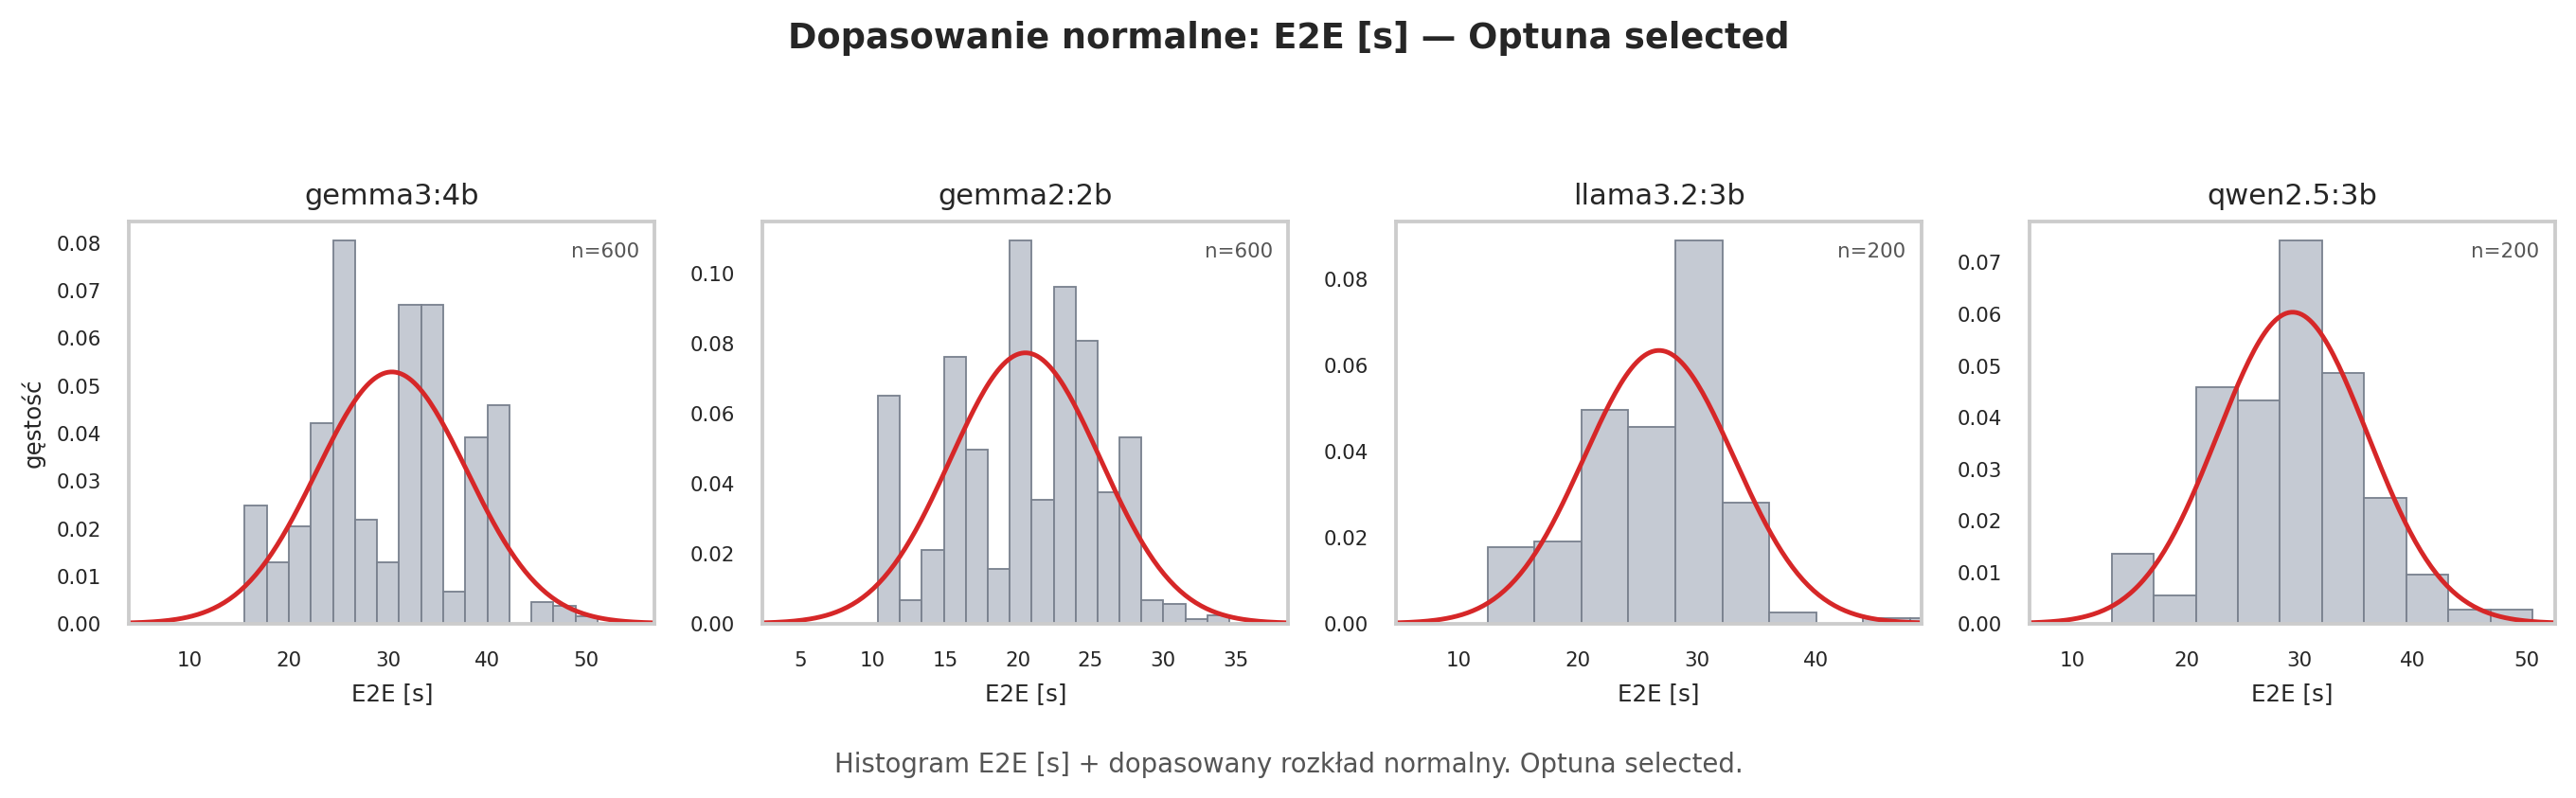
\includegraphics[width=0.95\textwidth]{optuna_e2e_gauss_fit_matrix.png}
  \caption{Dopasowanie rozkładu normalnego do opóźnienia E2E
           (\texttt{results-selected-9.05}). Histogram oraz gęstość
           $\mathcal{N}(\hat\mu,\hat\sigma^2)$ per model.}
  \label{fig:optuna_gauss_fit}
\end{figure}

Kompromis Pareto (rysunek~\ref{fig:pareto_latency_hall}) zestawia średnie E2E
($\pm\sigma$) ze wskaźnikiem halucynacji. Żaden model nie dominuje w~obu
wymiarach jednocześnie: \texttt{gemma2:2b} jest najszybszy
($\mathrm{E2E}\approx 20{,}5$~s), lecz ma ok.~18\%~halucynacji;
\texttt{gemma3:4b} jest wolniejszy ($\approx 30{,}4$~s), lecz osiąga
ok.~1{,}2\%~halucynacji. Dla asystenta informującego o~stanie domu błędna
informacja jest groźniejsza niż kilka sekund dłuższej odpowiedzi --- stąd
wybór \texttt{gemma3:4b} jako kandydata produkcyjnego. Rozsądny preset
hiperparametrów wystarcza; Optuna nie wskazuje silnie dominującej konfiguracji
jakościowej.

\begin{figure}[H]
  \centering
  
\includegraphics[width=0.85\textwidth]{04_latency_hallucination_pareto_selected.png}
  \caption{Kompromis Pareto: średnie opóźnienie E2E ($\pm\sigma$, model Gaussa)
           vs wskaźnik halucynacji (\texttt{results-selected-9.05}).
           Rozmiar punktu odpowiada średniemu \emph{composite score}.}
  \label{fig:pareto_latency_hall}
\end{figure}


% ============================================================
\subsection{Etap kwantyzacji: cold vs warm i model log-normalny}
\label{subsec:kwantyzacja}
% ============================================================

\subsubsection{Typy kwantyzacji GGUF}

Modele w~Ollamie przechowywane są w~formacie GGUF z~różnymi poziomami
kwantyzacji wag. W~badaniach uwzględniono cztery warianty:
\begin{itemize}
  \item \textbf{Q8\_0} --- 8-bitowe wagi bez grupowania; baseline,
  \item \textbf{Q4\_K\_M} --- 4-bitowe wagi z~grupowaniem K i~mixed precision~M,
  \item \textbf{Q4\_0} --- 4-bitowe wagi bez grupowania,
  \item \textbf{Q2\_K} --- 2-bitowe wagi z~grupowaniem; agresywna kompresja.
\end{itemize}
Mniejsza precyzja oznacza mniejszy plik i~mniej danych do przenoszenia
z~pamięci, co teoretycznie przyspiesza dekodowanie tokenów. Zbyt agresywna
kwantyzacja może jednak destabilizować generację.

\begin{table}[H]
  \centering
  \caption{Rozmiary plików GGUF [GB] dla badanych modeli.}
  \label{tab:gguf_rozmiary}
  \begin{tabular}{lcccc}
    \hline
    Model & Q2\_K & Q4\_0 & Q4\_K\_M & Q8\_0 \\
    \hline
    \texttt{gemma3-4b}   & 1{,}61 & 2{,}20 & 2{,}32 & 3{,}85 \\
    \texttt{gemma4-e2b}  & 2{,}78 & 3{,}13 & 3{,}19 & 4{,}63 \\
    \texttt{bielik-4.5b} & 1{,}65 & 2{,}52 & 2{,}68 & 4{,}71 \\
    \hline
  \end{tabular}
\end{table}

\subsubsection{Dlaczego pierwsze pomiary ``nic nie pokazywały''}

Przy zmiennym prompcie lub zimnym cache metryka E2E dla różnych wariantów
kwantyzacji wygląda podobnie, ponieważ
$\mathrm{E2E} = \mathrm{TTFT} + \mathrm{generation\_ms}$. TTFT (prefill)
zależy od długości promptu i~taktowania CPU, nie od precyzji wag. Kwantyzacja
wpływa przede wszystkim na \emph{generation\_ms}. Gdy TTFT dominuje budżet
czasu --- typowe przy cold cache --- różnice Q4/Q8 giną w~szumie E2E.
To wyjaśnia, dlaczego wczesne porównania ``po E2E'' nie dawały czytelnego
efektu kwantyzacji.

\subsubsection{Cold vs warm: izolacja generation\_ms}

Aby wyizolować czas generacji, zastosowano protokół \emph{warm-cache}:
stały \emph{system\_prompt}, \texttt{keep\_alive=30m}, \texttt{streaming=True},
\emph{generation\_ms} $= \mathrm{e2e\_ms} - \mathrm{ttft\_ms}$ per rekord.
Równolegle zebrano pomiary \emph{cold-cache} ($n\approx 100$ per komórka
model$\times$wariant). Rysunki~\ref{fig:dekompozycja_e2e}
i~\ref{fig:cold_dekompozycja_e2e} pokazują dekompozycję E2E na TTFT i~generację
jako mediany modelu log-normalnego~$e^{\hat\mu}$.

\begin{figure}[H]
  \centering
  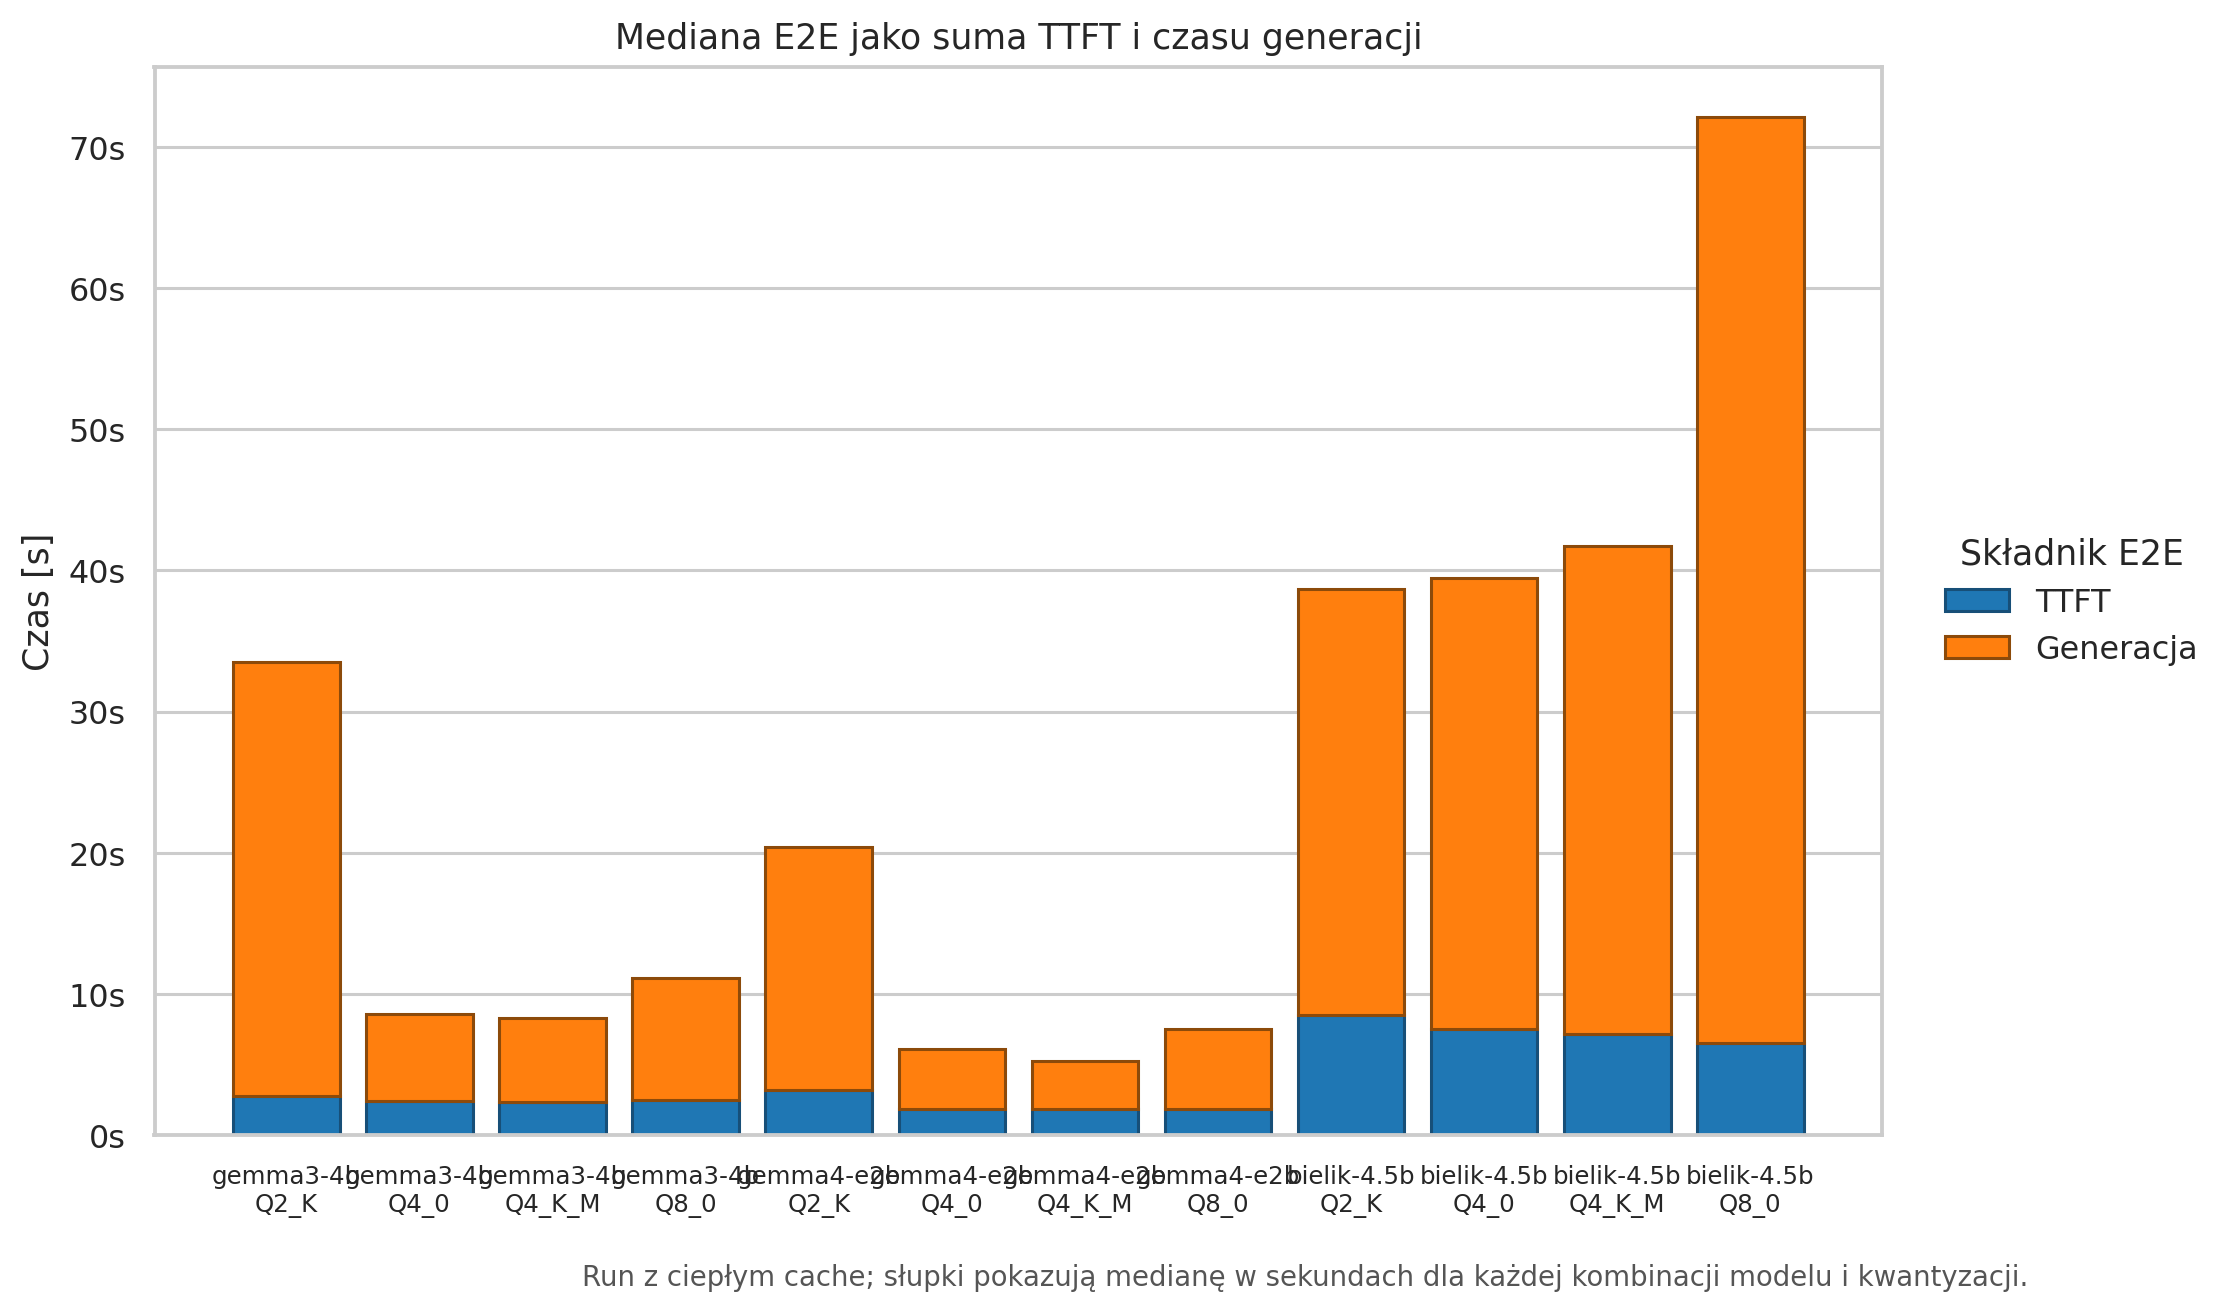
\includegraphics[width=0.95\textwidth]{03_dekompozycja_e2e.png}
  \caption{Dekompozycja E2E na TTFT i~\emph{generation\_ms} (warm cache).
           Wysokości słupków to mediany modelu log-normalnego $e^{\hat\mu}$
           ($n\approx 100$). Kwantyzacja wpływa głównie na czas generacji.}
  \label{fig:dekompozycja_e2e}
\end{figure}

\begin{figure}[H]
  \centering
  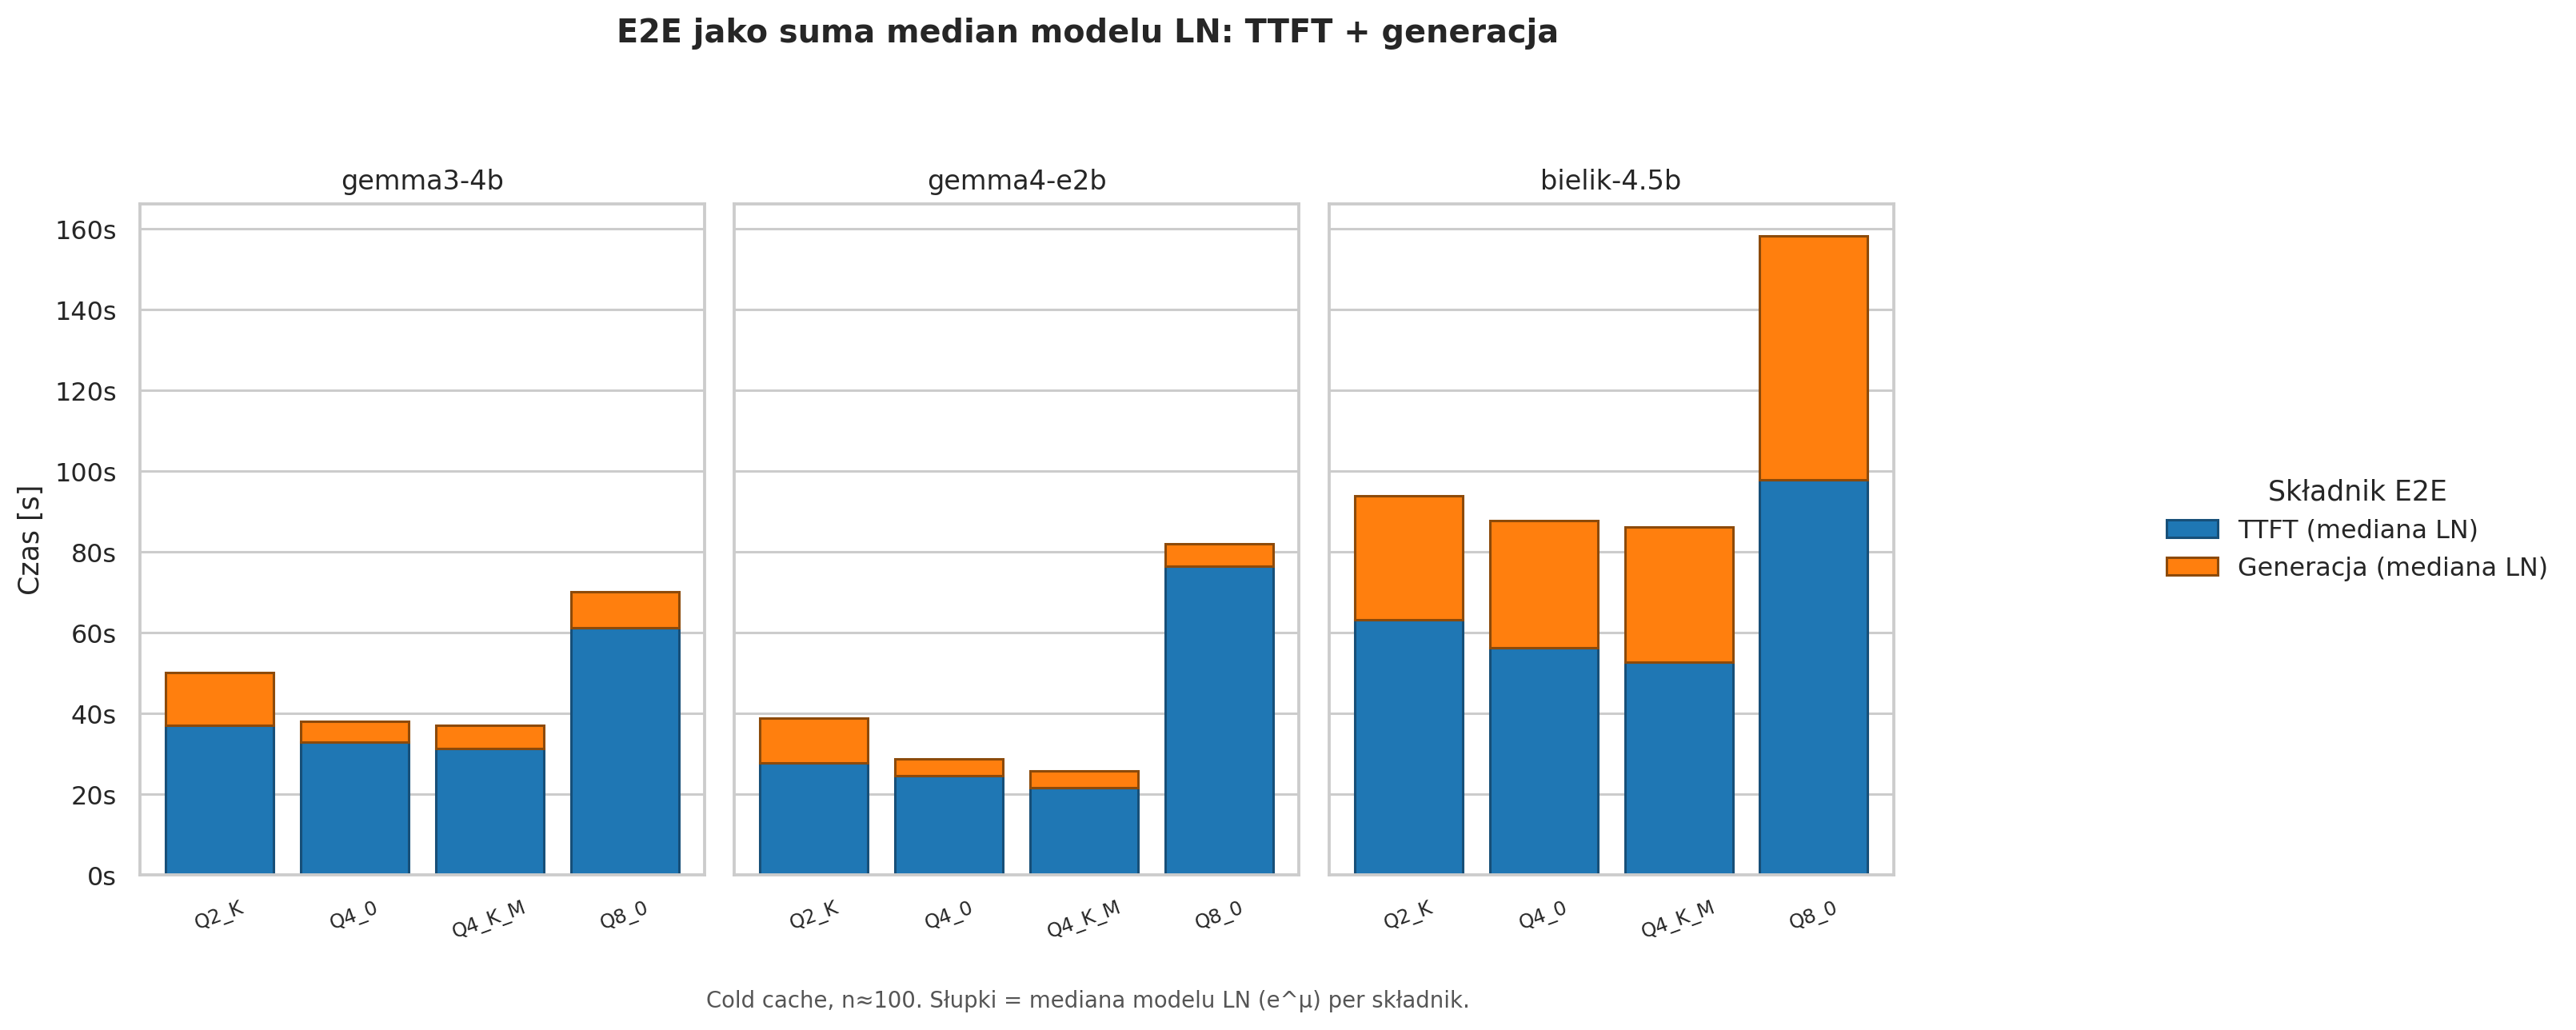
\includegraphics[width=0.95\textwidth]{cold_03_dekompozycja_e2e.png}
  \caption{Dekompozycja E2E na TTFT i~\emph{generation\_ms} (cold cache).
           Mediany modelu LN $e^{\hat\mu}$, $n\approx 100$. Prefill dominuje
           budżet czasu.}
  \label{fig:cold_dekompozycja_e2e}
\end{figure}

\subsubsection{Model log-normalny dla czasów generacji}

Czasy generacji są dodatnie i~prawostronnie skośne (różna długość odpowiedzi).
Przyjęto więc wspólny model roboczy log-normalny: lokalizacja
$e^{\hat\mu}$ (mediana modelu LN), przedział $e^{\hat\mu\pm\hat\sigma}$.
Rysunek~\ref{fig:warm_ln_fit} pokazuje histogramy \emph{generation} oraz
dopasowaną gęstość LN dla warm cache (analogicznie cold ---
rysunek~\ref{fig:cold_ln_fit}).

\begin{figure}[H]
  \centering
  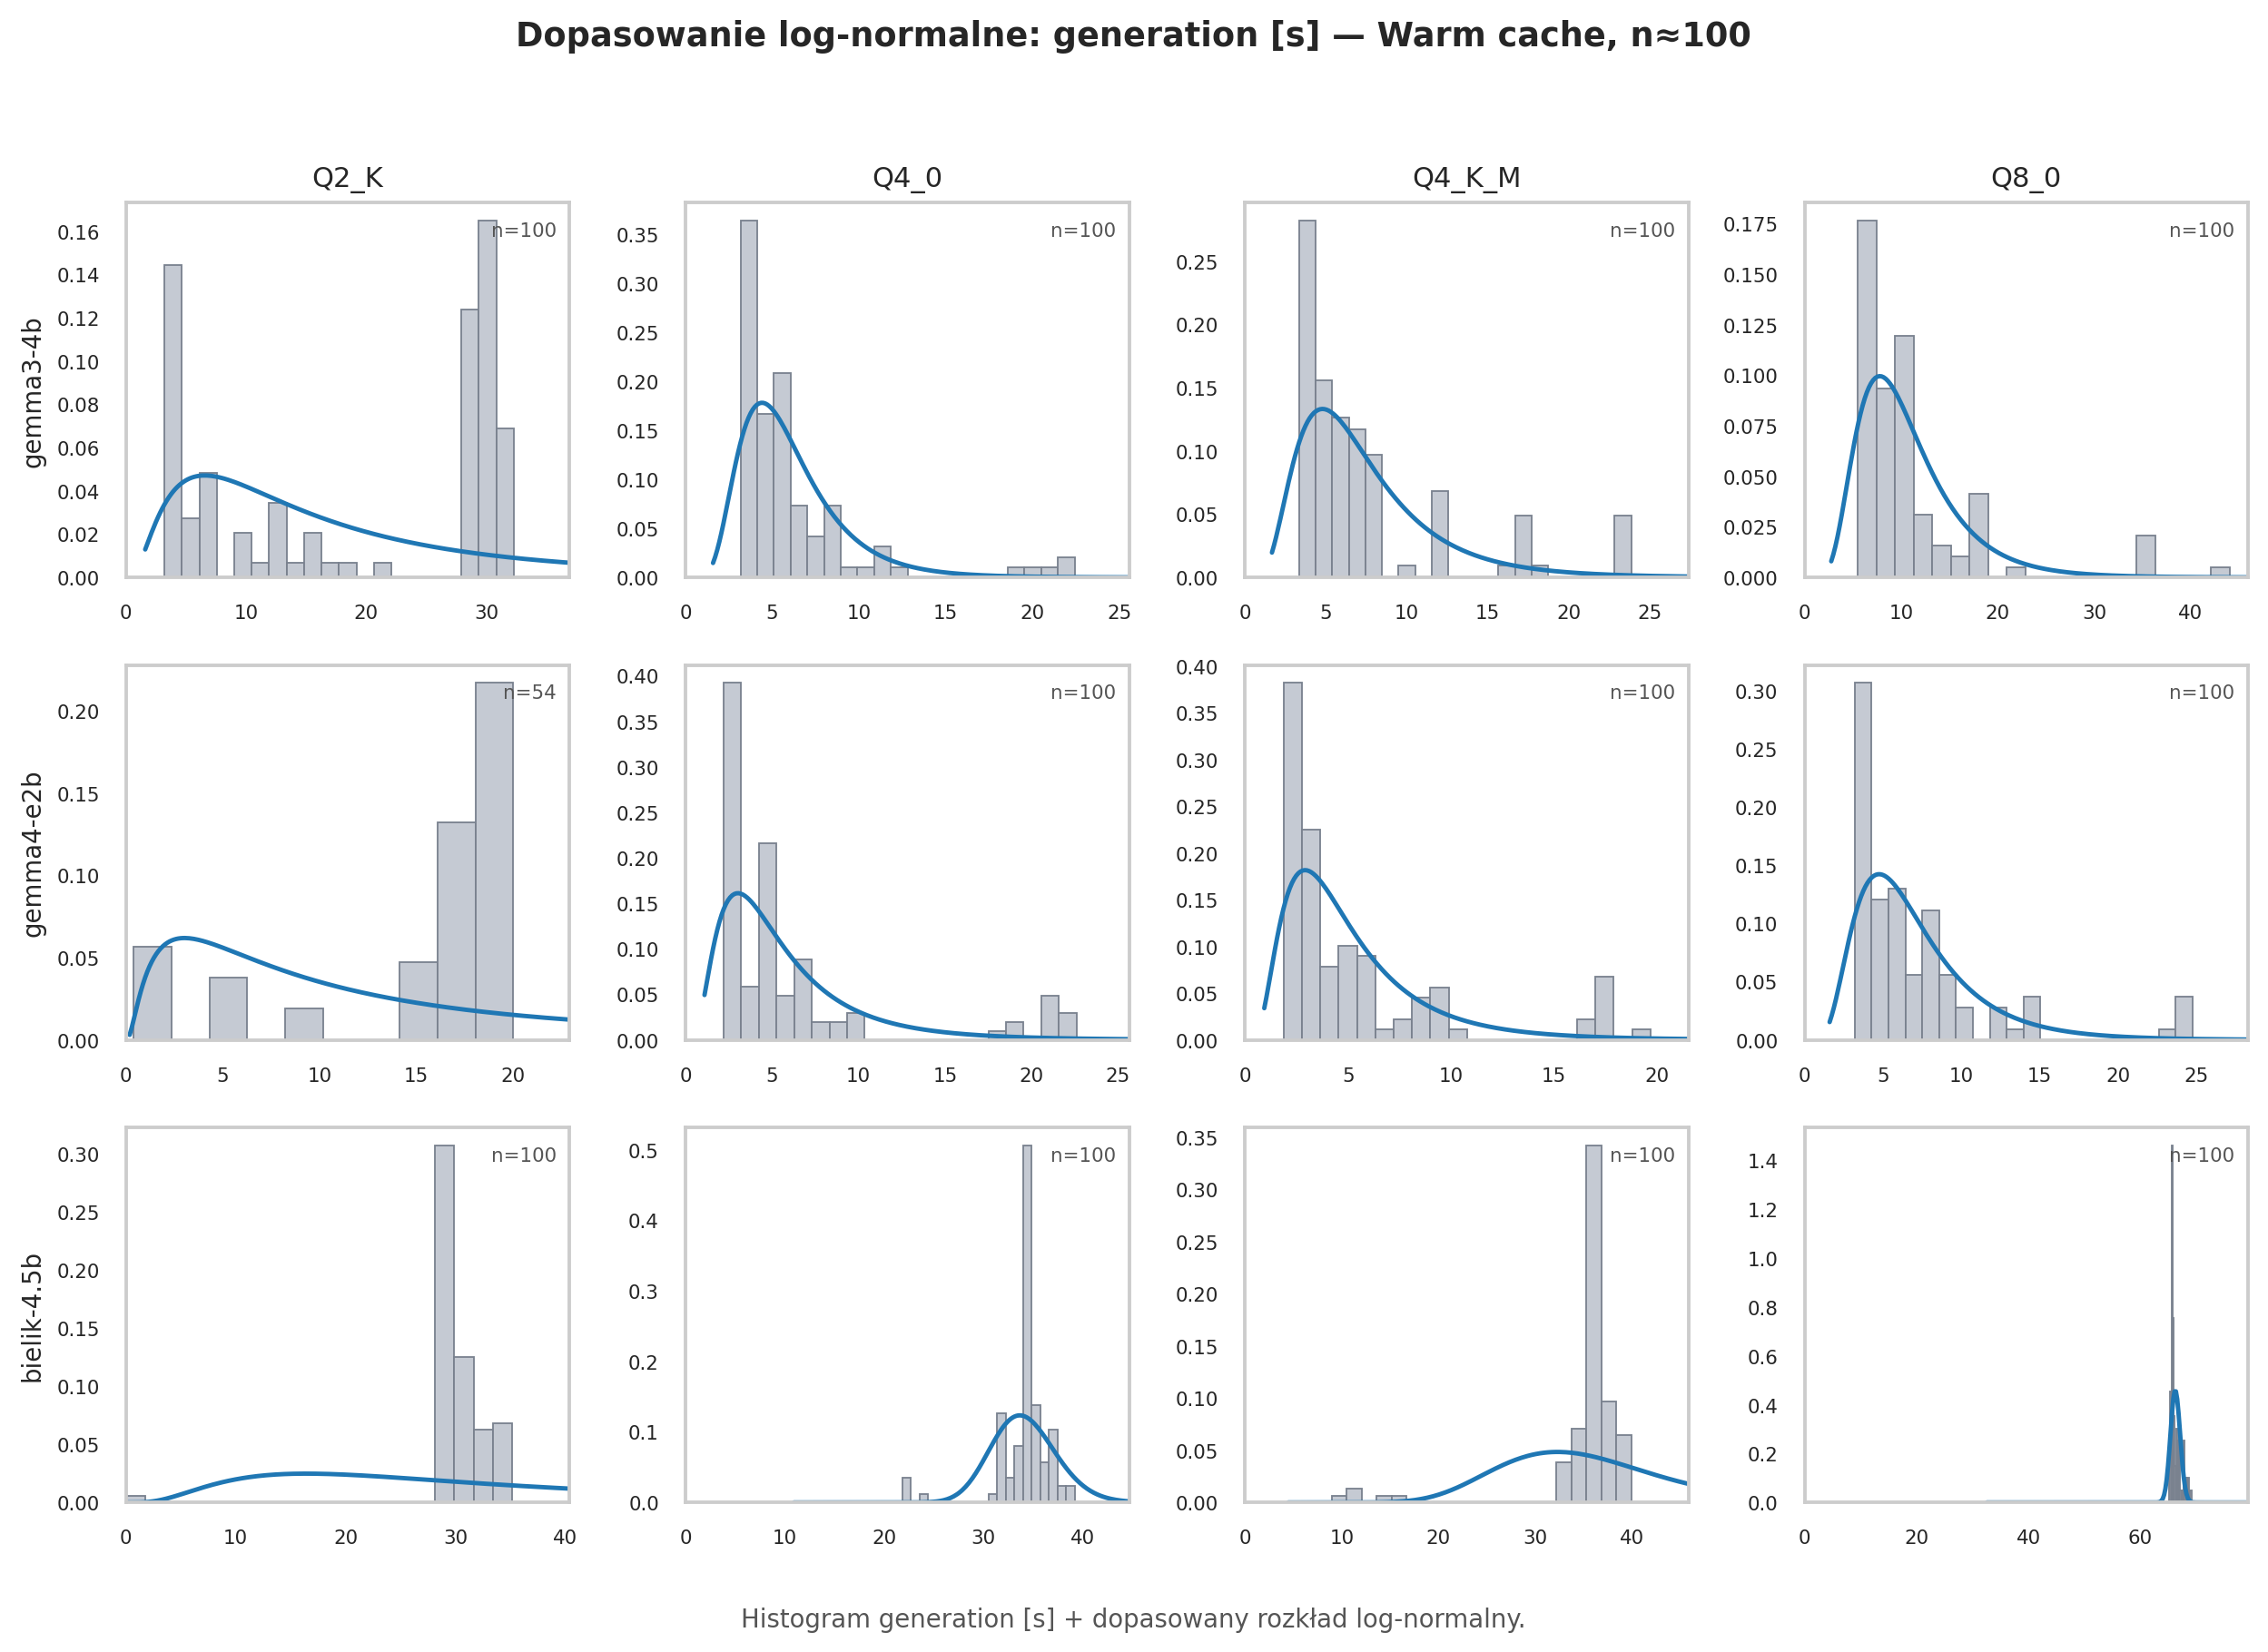
\includegraphics[width=0.95\textwidth]{warm_generation_ln_fit_matrix.png}
  \caption{Dopasowanie rozkładu log-normalnego do \emph{generation\_ms}
           (warm cache, $n\approx 100$). Histogram oraz gęstość LN per model
           i~wariant kwantyzacji.}
  \label{fig:warm_ln_fit}
\end{figure}

\begin{figure}[H]
  \centering
  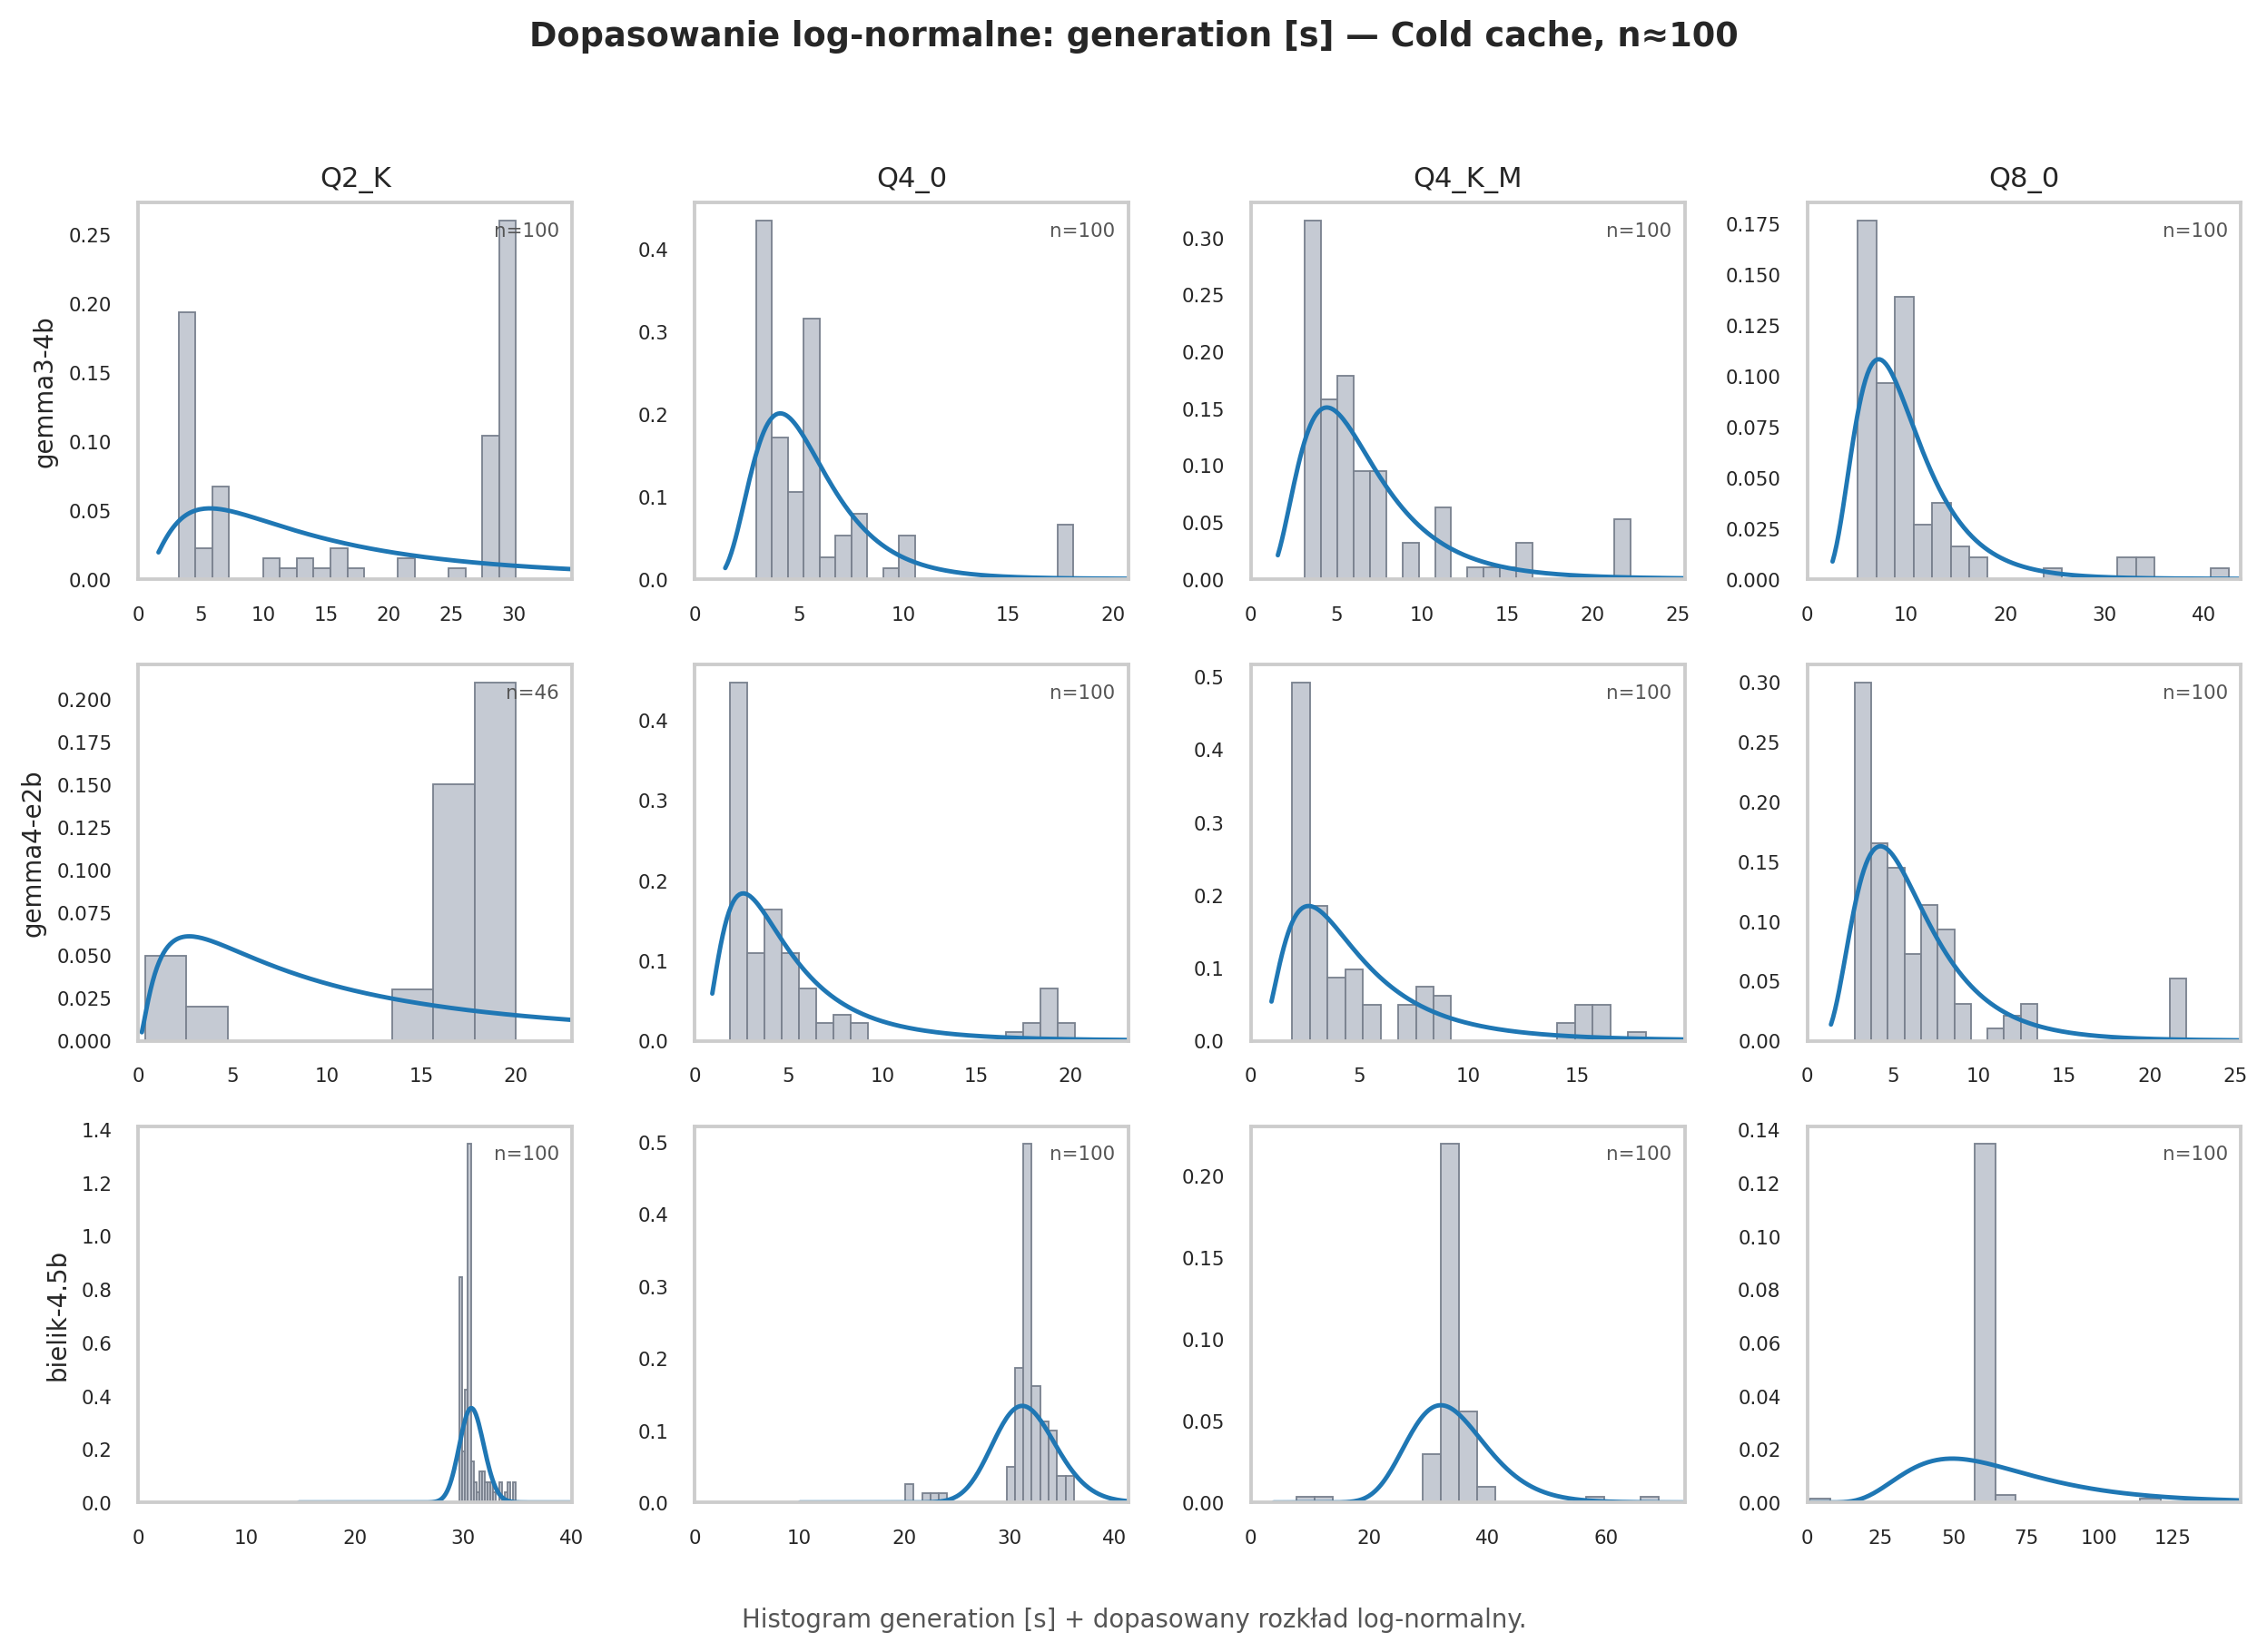
\includegraphics[width=0.95\textwidth]{cold_generation_ln_fit_matrix.png}
  \caption{Dopasowanie rozkładu log-normalnego do \emph{generation\_ms}
           (cold cache, $n\approx 100$).}
  \label{fig:cold_ln_fit}
\end{figure}

\subsubsection{Wyniki warm-cache}

Tabela~\ref{tab:kwantyzacja_wyniki} zestawia mediany modelu LN dla TTFT,
generacji i~E2E oraz przyspieszenie generacji względem Q8\_0
($\mathrm{speedup}= e^{\hat\mu_{\mathrm{Q8}}}/e^{\hat\mu_{\mathrm{wariant}}}$).

\begin{table}[H]
  \centering
  \caption{Wyniki kwantyzacji warm-cache: mediany modelu LN ($e^{\hat\mu}$)
           oraz przyspieszenie generacji względem Q8\_0 ($n\approx 100$).}
  \label{tab:kwantyzacja_wyniki}
  \small
  \begin{tabular}{llccccc}
    \hline
    Model & Wariant & GGUF & TTFT & Gen & E2E & Speedup \\
    \hline
    \texttt{gemma3-4b}  & Q2\_K   & 1{,}61G & 2{,}74s & 14{,}18s & 17{,}74s & 0{,}68$\times$ \\
    \texttt{gemma3-4b}  & Q4\_0   & 2{,}20G & 2{,}52s & 5{,}44s  & 8{,}06s  & 1{,}77$\times$ \\
    \texttt{gemma3-4b}  & Q4\_K\_M& 2{,}32G & 2{,}44s & 6{,}42s  & 9{,}02s  & 1{,}50$\times$ \\
    \texttt{gemma3-4b}  & Q8\_0   & 3{,}85G & 2{,}51s & 9{,}66s  & 12{,}30s & 1{,}00$\times$ \\
    \texttt{gemma4-e2b} & Q2\_K   & 2{,}78G & 3{,}08s & 10{,}79s & 16{,}44s & 0{,}57$\times$ \\
    \texttt{gemma4-e2b} & Q4\_0   & 3{,}13G & 1{,}93s & 4{,}67s  & 6{,}80s  & 1{,}33$\times$ \\
    \texttt{gemma4-e2b} & Q4\_K\_M& 3{,}19G & 1{,}83s & 4{,}29s  & 6{,}30s  & 1{,}45$\times$ \\
    \texttt{gemma4-e2b} & Q8\_0   & 4{,}63G & 1{,}88s & 6{,}20s  & 8{,}22s  & 1{,}00$\times$ \\
    \texttt{bielik-4.5b}& Q2\_K   & 1{,}65G & 8{,}58s & 28{,}51s & 39{,}19s & 2{,}32$\times$ \\
    \texttt{bielik-4.5b}& Q4\_0   & 2{,}52G & 7{,}59s & 34{,}00s & 41{,}64s & 1{,}95$\times$ \\
    \texttt{bielik-4.5b}& Q4\_K\_M& 2{,}68G & 7{,}06s & 34{,}36s & 41{,}67s & 1{,}93$\times$ \\
    \texttt{bielik-4.5b}& Q8\_0   & 4{,}71G & 6{,}54s & 66{,}22s & 72{,}78s & 1{,}00$\times$ \\
    \hline
  \end{tabular}
\end{table}

\begin{figure}[H]
  \centering
  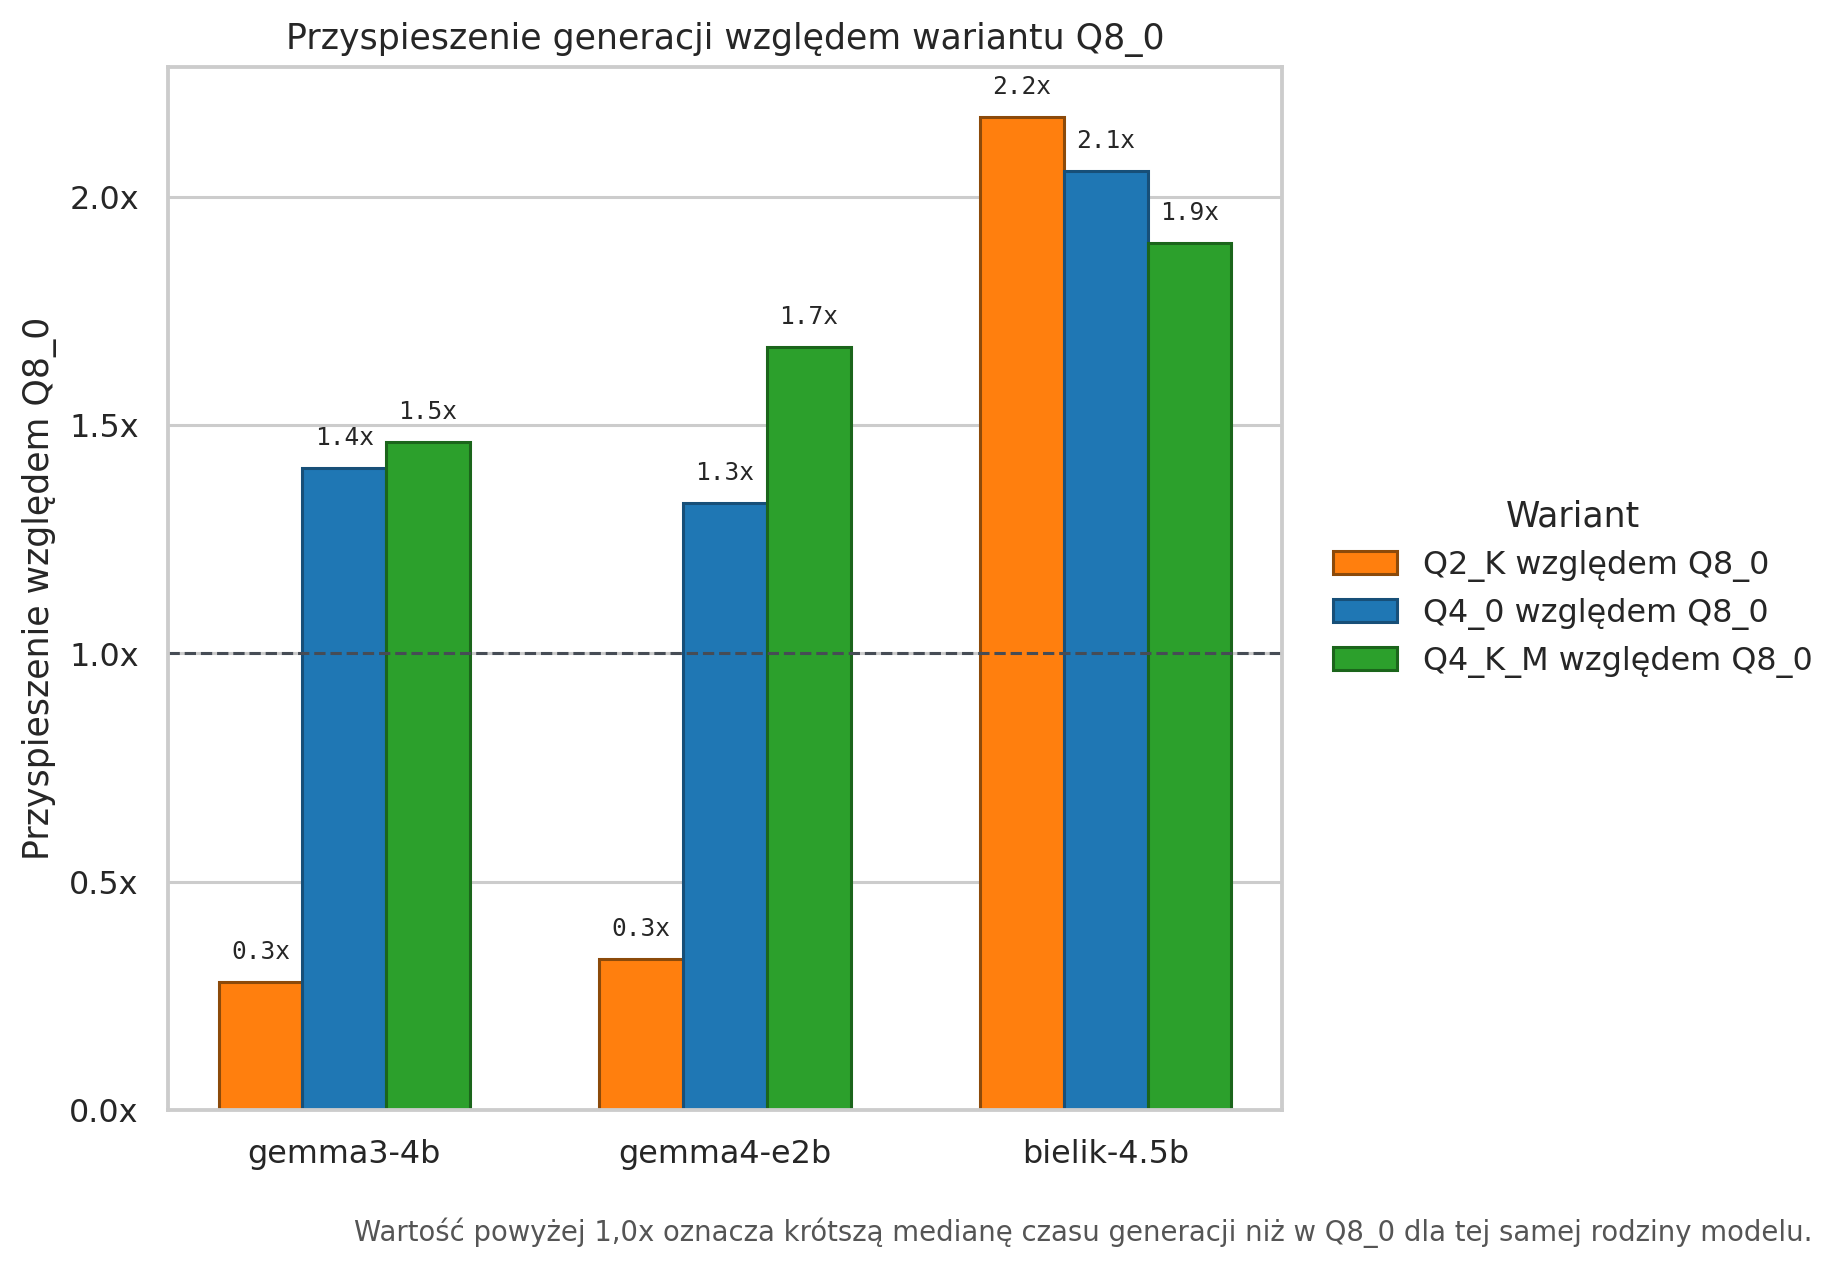
\includegraphics[width=0.85\textwidth]{04_przyspieszenie_wzgledem_q8.png}
  \caption{Przyspieszenie \emph{generation\_ms} względem Q8\_0 (warm cache).
           Speedup $= e^{\hat\mu_{\mathrm{Q8}}}/e^{\hat\mu_{\mathrm{wariant}}}$.}
  \label{fig:speedup_q8}
\end{figure}

\begin{figure}[H]
  \centering
  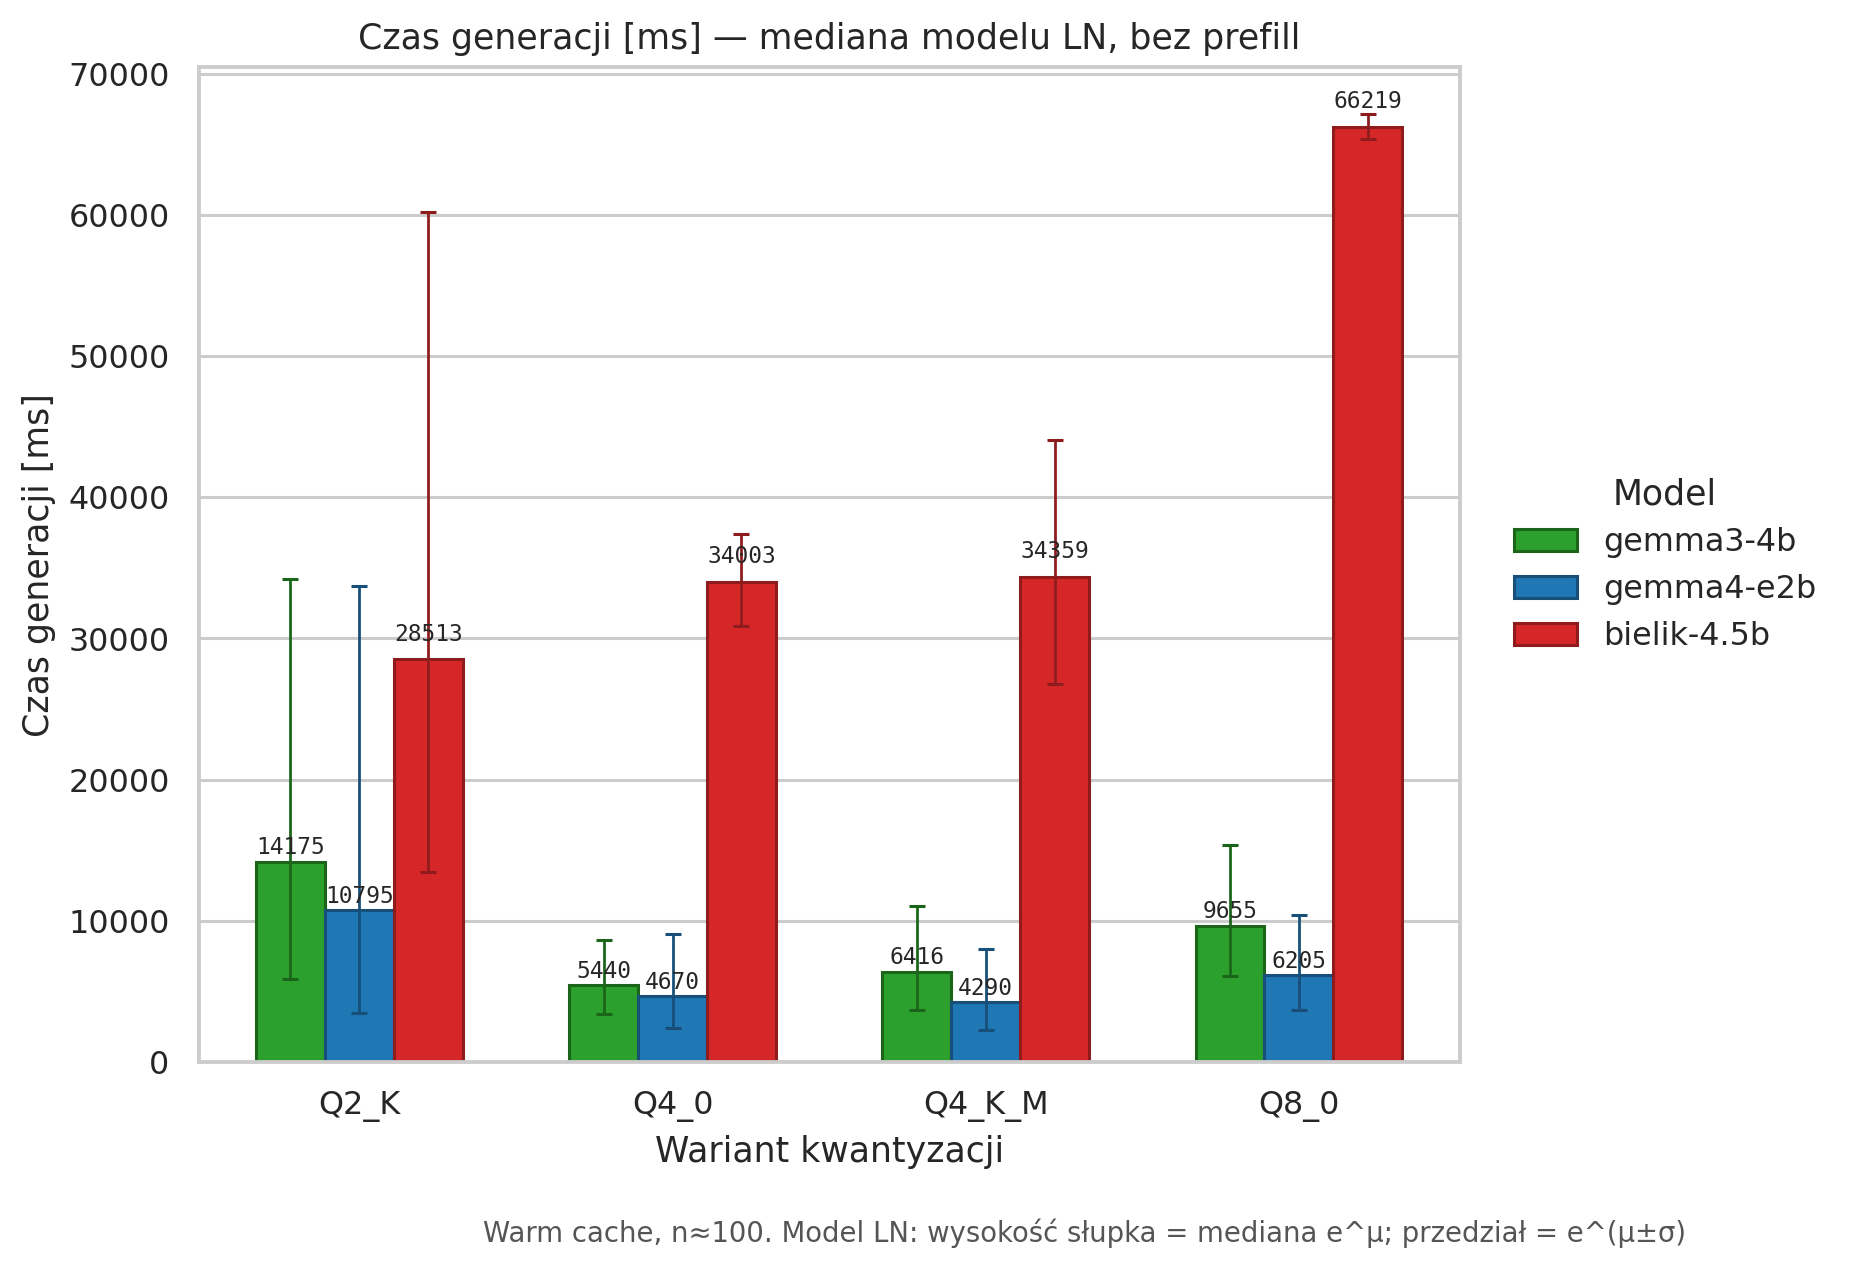
\includegraphics[width=0.85\textwidth]{07_generation_ms_wedlug_wariantu.png}
  \caption{Czas \emph{generation\_ms} według wariantu kwantyzacji
           (mediana modelu LN $e^{\hat\mu}$, przedział $e^{\hat\mu\pm\hat\sigma}$;
           warm cache, $n\approx 100$).}
  \label{fig:gen_ms_variant}
\end{figure}

\begin{figure}[H]
  \centering
  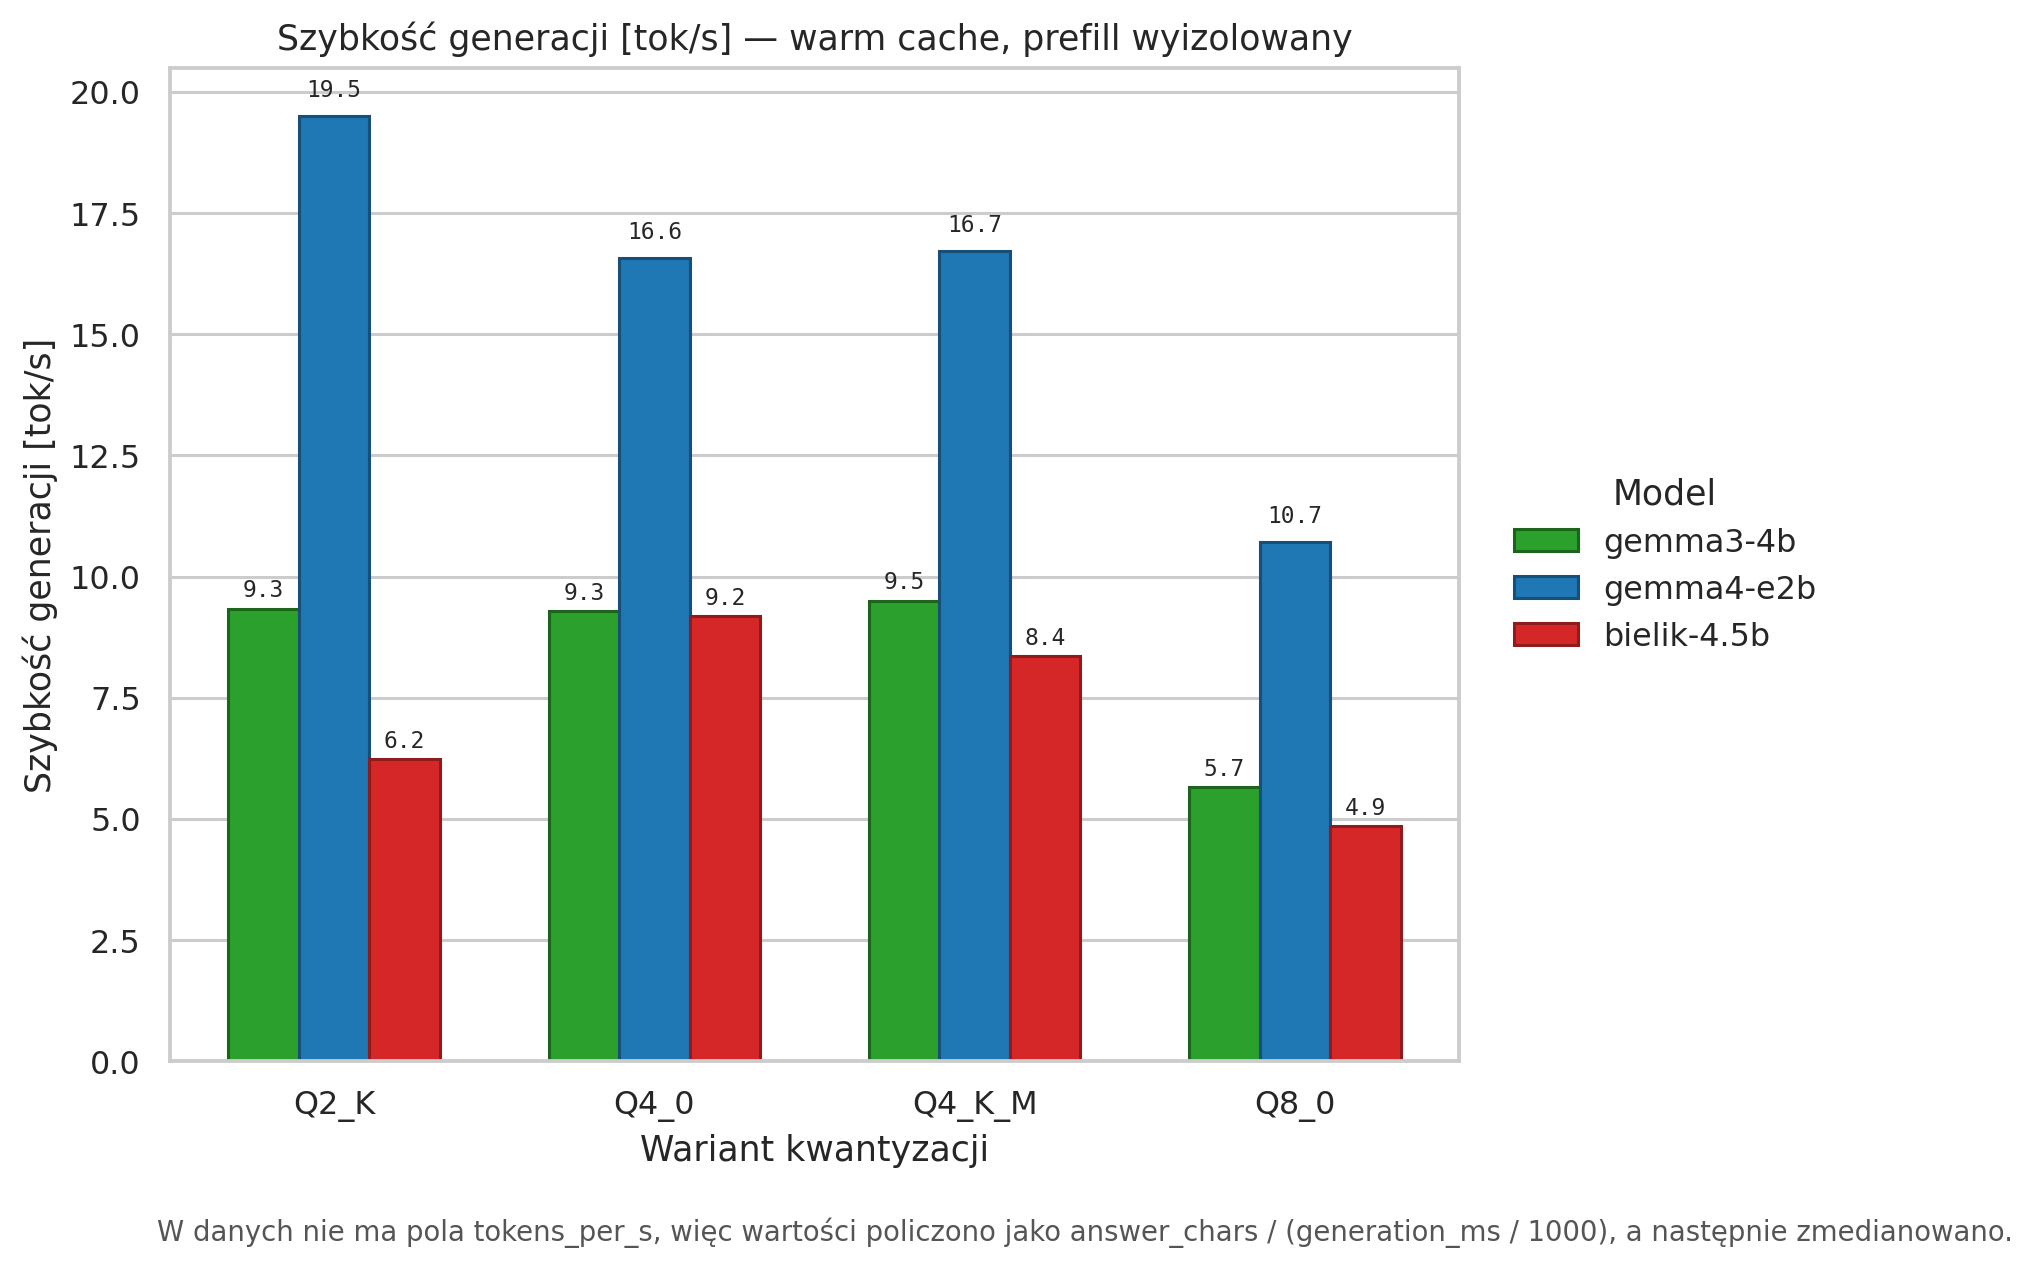
\includegraphics[width=0.85\textwidth]{08_szybkosc_generacji_tok_s_wedlug_wariantu.png}
  \caption{Szybkość generacji [znaki/s] (proxy tok/s) według wariantu
           kwantyzacji. Mediana modelu LN na per-rekord
           $\mathrm{answer\_chars}/(\mathrm{generation\_ms}/1000)$.}
  \label{fig:tok_s_variant}
\end{figure}

\subsubsection{Anomalie i wnioski}
\label{subsubsec:anomalie}

\textbf{Anomalia Q2\_K.} Wariant \texttt{gemma3-4b/Q2\_K} ma długi czas
generacji mimo małego pliku GGUF: przy niskiej precyzji wag model produkuje
rozwlekłe odpowiedzi (rysunek~\ref{fig:gen_vs_length}).

\begin{figure}[H]
  \centering
  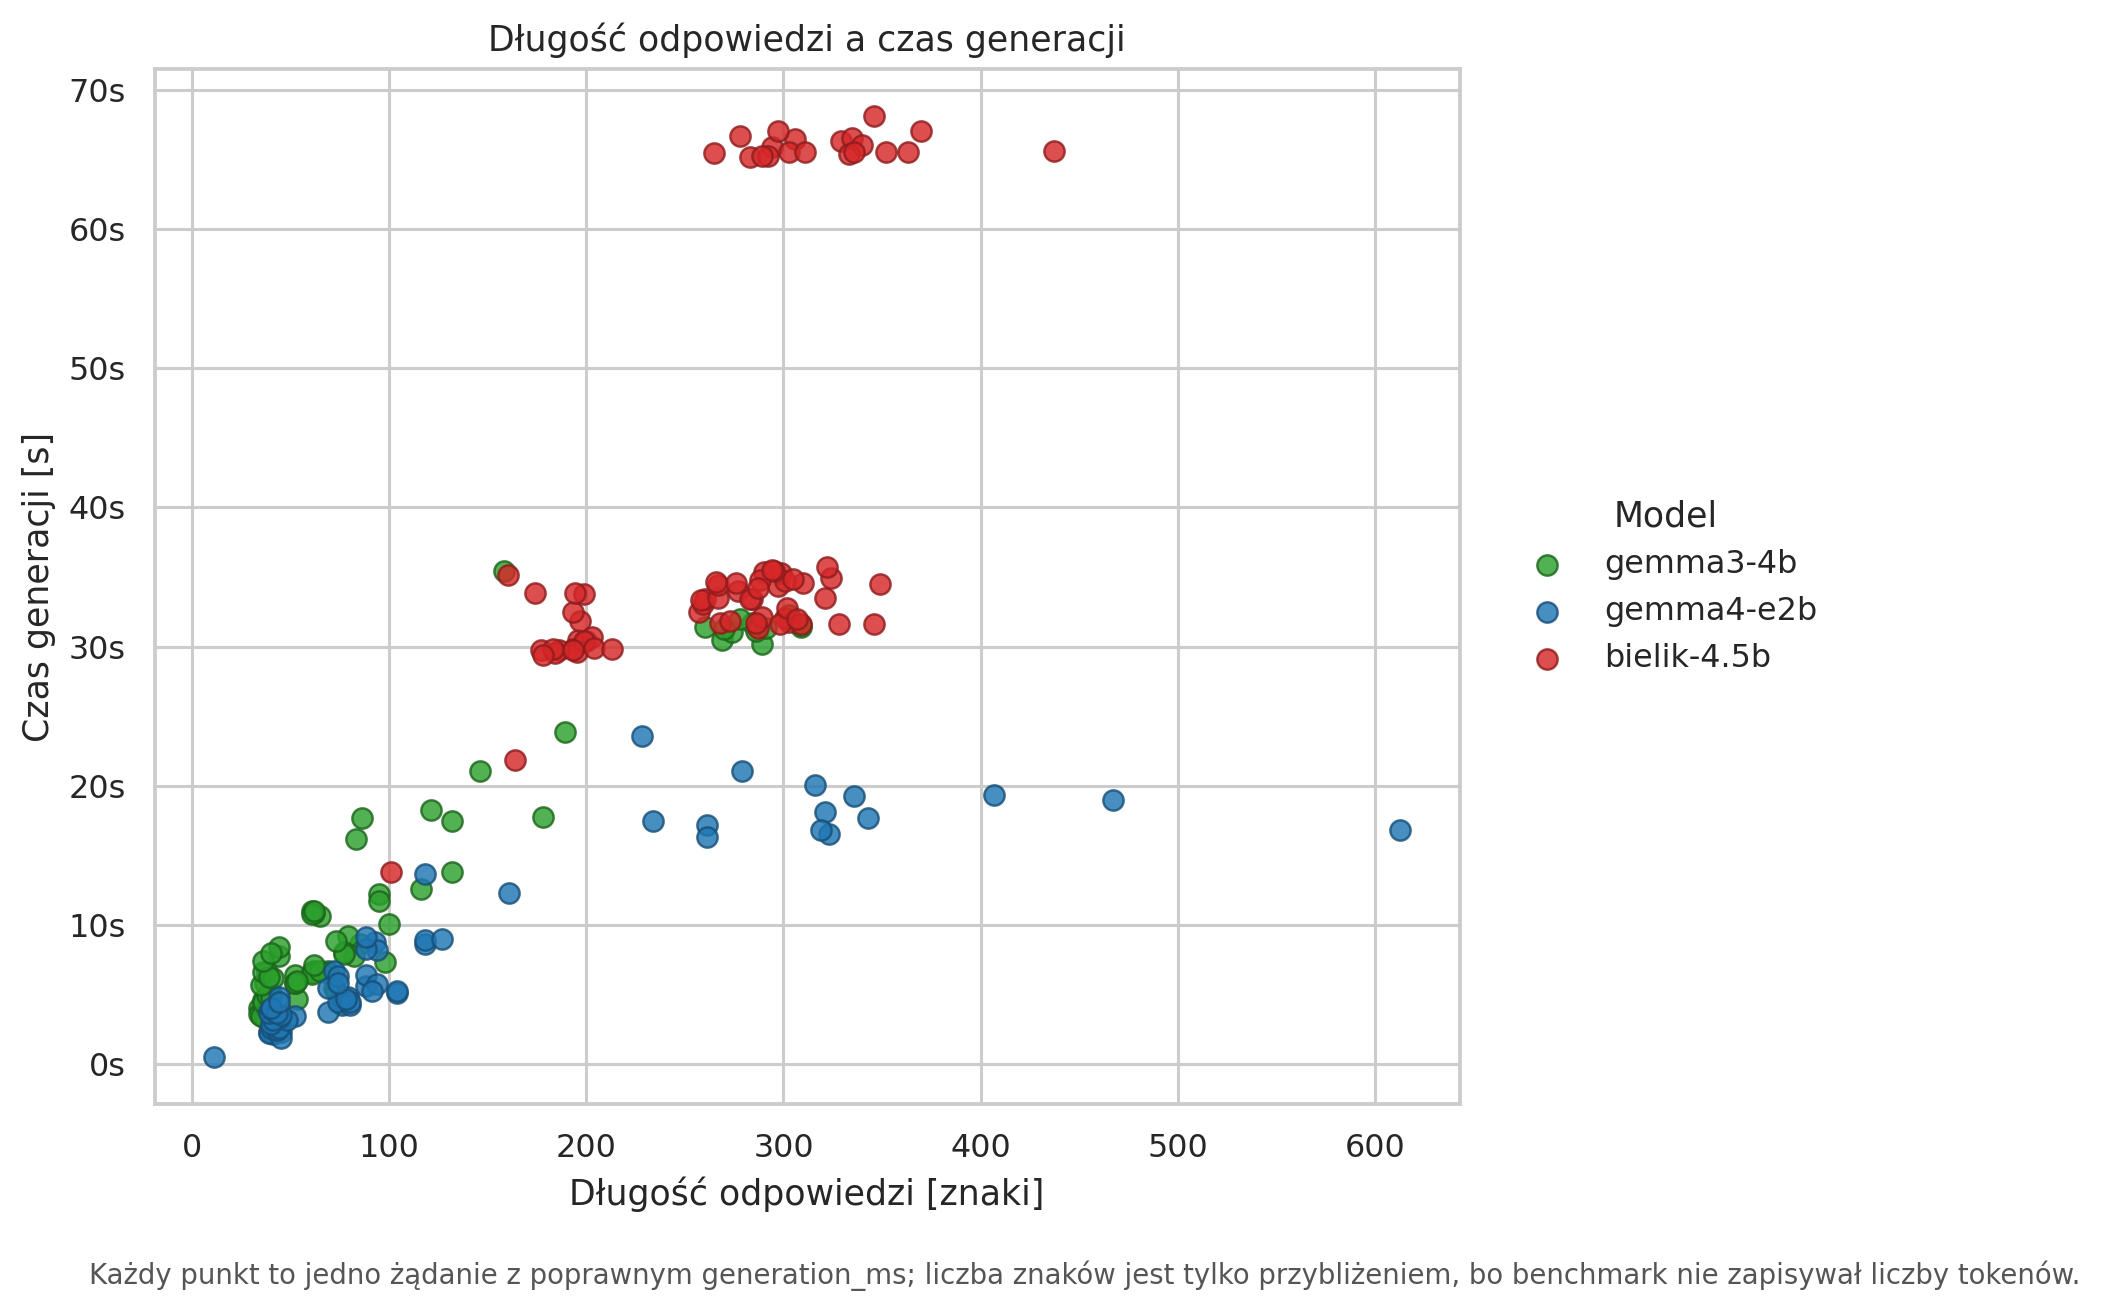
\includegraphics[width=0.85\textwidth]{05_generacja_a_dlugosc_odpowiedzi.png}
  \caption{Zależność czasu generacji od długości odpowiedzi
           (anomalia Q2\_K; warm cache).}
  \label{fig:gen_vs_length}
\end{figure}

\textbf{Anomalia \texttt{gemma4-e2b/Q2\_K}.} Model MoE jest wrażliwy na
kwantyzację 2-bitową (część pustych odpowiedzi / niższy hit rate cache).

\textbf{Odrzucenie Bielika.} Nawet przy Q4\_K\_M mediana LN generacji wynosi
ok.~34~s --- rzędu $5\times$ wolniej niż \texttt{gemma3-4b/Q4\_K\_M}. Model
nie jest wariantem produkcyjnym dla asystenta głosowego w~tym środowisku.

\textbf{Wniosek.} Q4\_K\_M to sensowny kompromis dla Gemm: dla
\texttt{gemma3-4b} ok.~$1{,}50\times$ przyspieszenie generacji względem Q8\_0
przy mniejszym pliku; dla \texttt{gemma4-e2b} ok.~$1{,}45\times$. Kwantyzacja
nie redukuje halucynacji --- to własność wag, nie precyzji reprezentacji.
Dalsza dźwignia opóźnienia to redukcja TTFT przez układanie promptu pod
\emph{prefix caching} (sekcja~\ref{subsec:prefix_caching}).


% ============================================================
\subsection{Prompt engineering i prefix caching}
\label{subsec:prefix_caching}
% ============================================================

\subsubsection{Problem: TTFT przy długim prompcie}

W~systemie Wilga \emph{system\_prompt} zawiera statyczny nagłówek (reguły,
instrukcje), blok sensoryczny oraz kontekst nauczyciela. Przy każdym zapytaniu
z~nowym kontekstem sensorycznym urządzenie musi wykonać prefill od zera.
W~protokole cold cache TTFT stanowi większość E2E; w~warm cache --- przy
stałym prefiksie --- TTFT spada o~rząd wielkości.

\subsubsection{Mechanizm prefix cachingu}

Podczas prefill model oblicza klucze~(K) i~wartości~(V). KV-cache może zostać
zachowane, jeśli tokeny od początku promptu są identyczne. Implikacja dla
architektury Teacher-Student (rozdział~3): statyczny blok musi być prefiksem,
a~zmienny (sensory, insight, pytanie) --- sufiksem.

\subsubsection{Empirycznie: cold vs warm TTFT}

Dla \texttt{gemma3-4b/Q4\_K\_M} mediana modelu LN TTFT wynosi ok.~31{,}3~s
w~cold cache oraz ok.~2{,}44~s w~warm cache
(rysunki~\ref{fig:cold_ttft},~\ref{fig:ttft_warm}). Redukcja
$(31{,}3 - 2{,}44)/31{,}3 \approx 92\%$. Porównanie dotyczy protokołów
cold vs warm przy tej samej siatce model$\times$wariant ($n\approx 100$).

\begin{figure}[H]
  \centering
  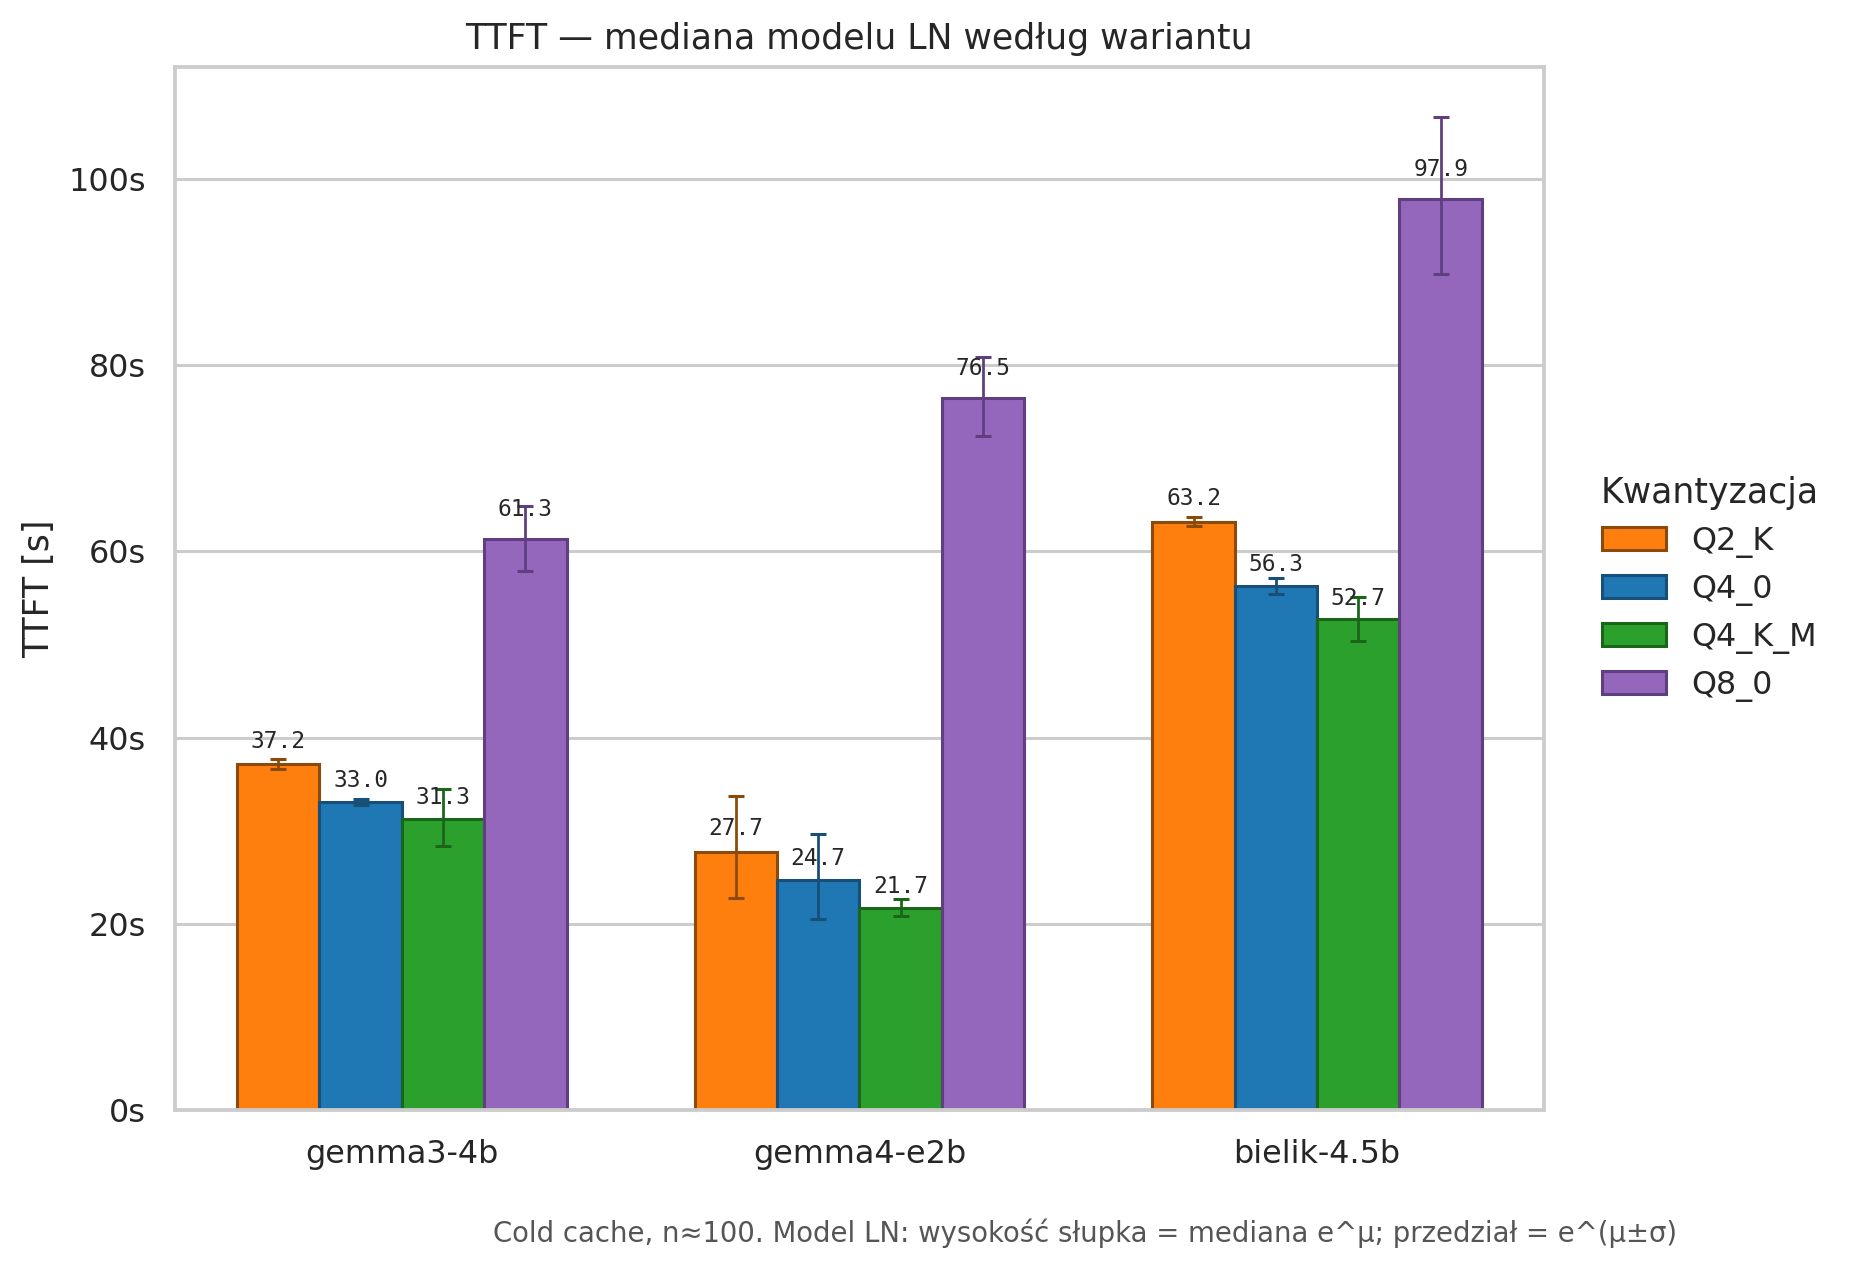
\includegraphics[width=0.85\textwidth]{cold_02_ttft_wedlug_wariantu.png}
  \caption{TTFT według wariantu kwantyzacji (cold cache):
           mediana modelu LN $e^{\hat\mu}$ z~przedziałem $e^{\hat\mu\pm\hat\sigma}$.}
  \label{fig:cold_ttft}
\end{figure}

\begin{figure}[H]
  \centering
  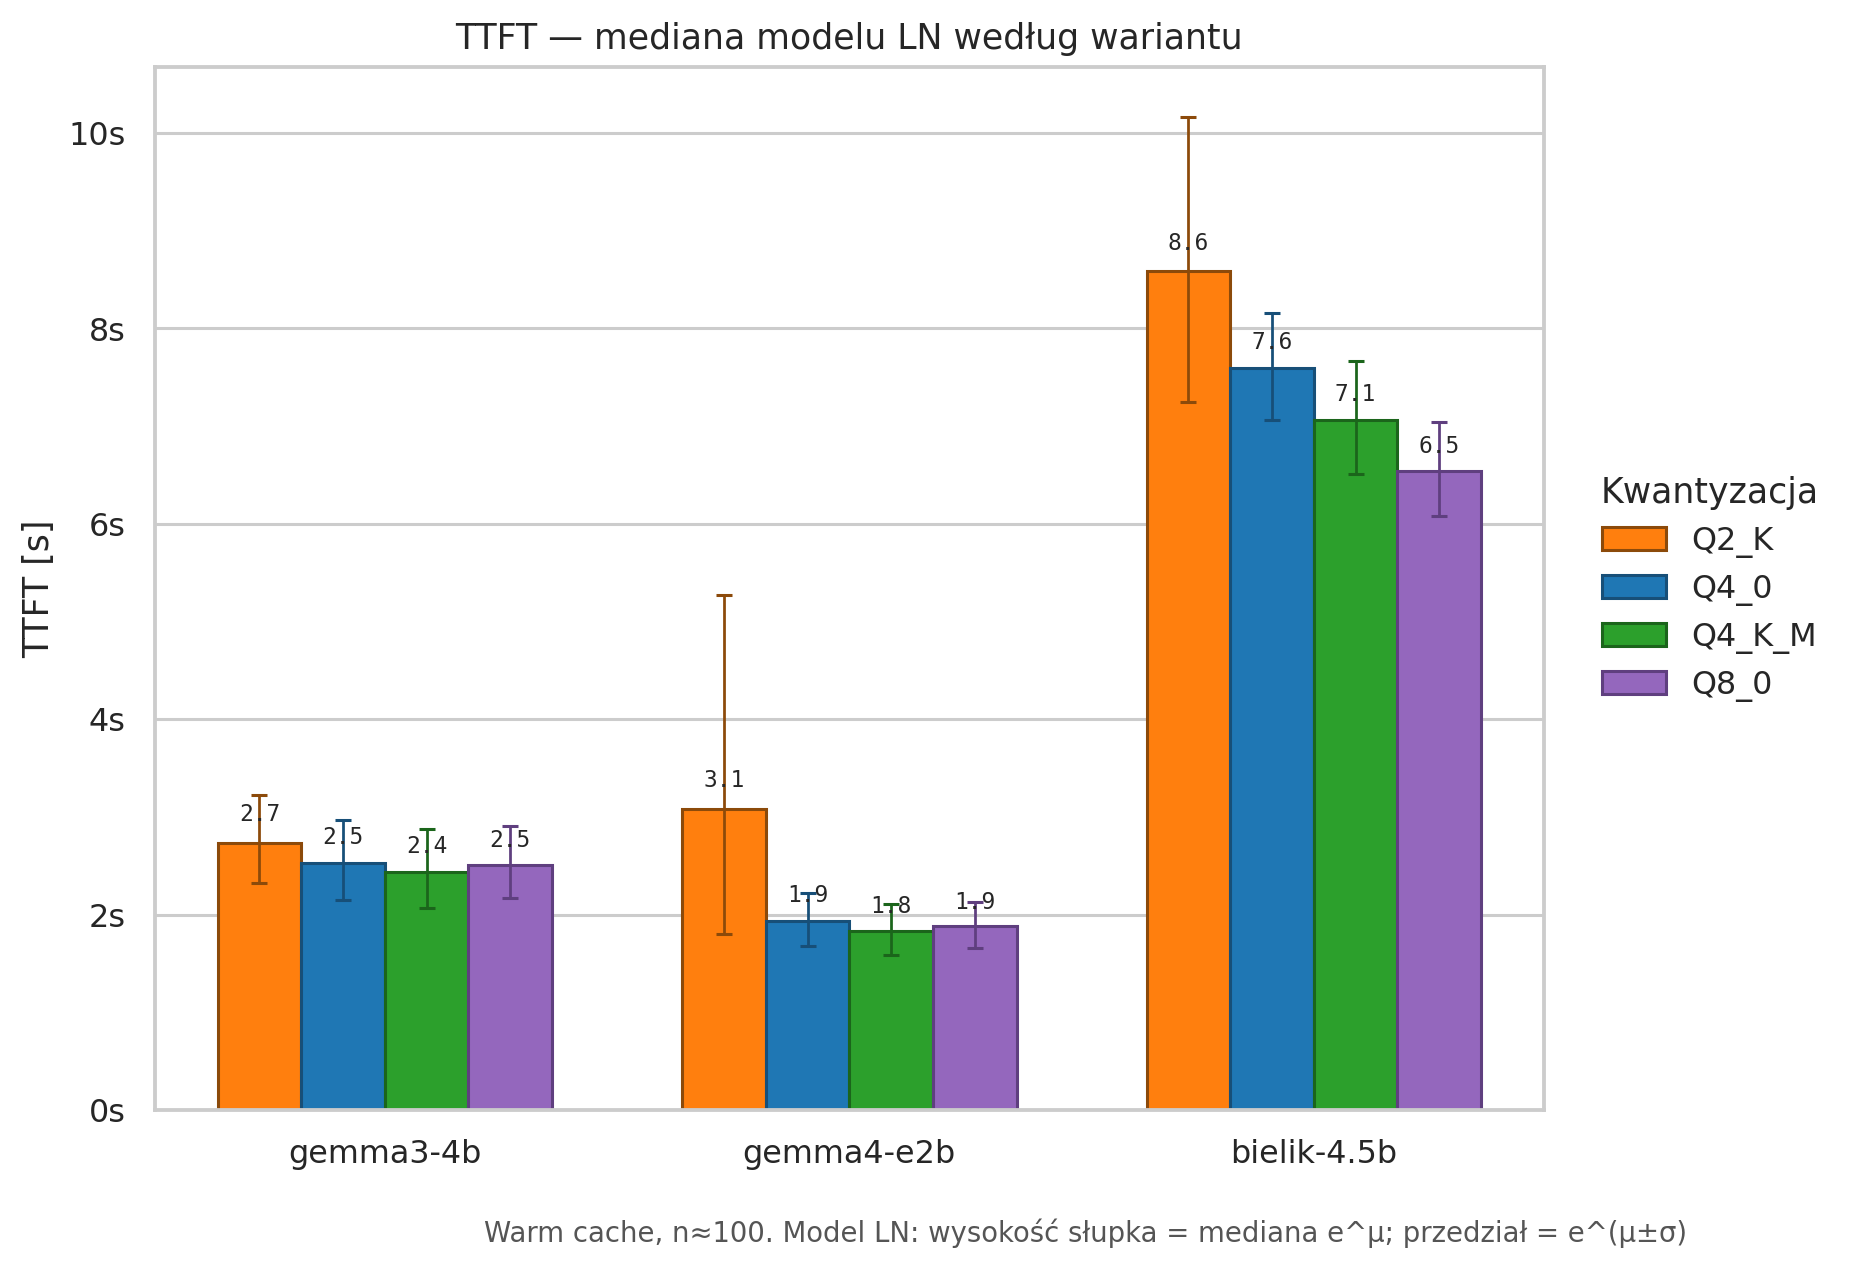
\includegraphics[width=0.85\textwidth]{02_ttft_wedlug_wariantu.png}
  \caption{TTFT według wariantu kwantyzacji (warm cache):
           mediana modelu LN $e^{\hat\mu}$ z~przedziałem $e^{\hat\mu\pm\hat\sigma}$.}
  \label{fig:ttft_warm}
\end{figure}

\subsubsection{Konsekwencje dla promptu Wilga}

Architektura promptu pod \emph{prefix caching}:
\begin{itemize}
  \item \textbf{[STATYCZNY PREFIKS]:} instrukcje, reguły (brak danych
        $\rightarrow$ przyznaj wprost), format odpowiedzi,
  \item \textbf{[DYNAMICZNY SUFIKS]:} dane sensoryczne, kontekst nauczyciela,
        pytanie użytkownika.
\end{itemize}
Po wdrożeniu \emph{prefix caching} i~kwantyzacji Q4\_K\_M dla
\texttt{gemma3-4b}: TTFT $\approx 2{,}4$~s, generacja $\approx 6{,}4$~s,
E2E $\approx 9$~s (mediany modelu LN, warm) --- akceptowalne dla asystenta
głosowego względem cold E2E rzędu kilkudziesięciu sekund.


% ============================================================
\subsection{Analiza wyników i rekomendacja produkcyjna}
\label{subsec:rekomendacja}
% ============================================================

\subsubsection{Porównanie modeli: wyniki końcowe}

Tabela~\ref{tab:wyniki_finalne} zestawia wyniki Optuny
(\texttt{results-selected-9.05}) z~95\%-owymi przedziałami ufności score
i~halucynacji (bootstrap) oraz średnim E2E~$\pm\sigma$ (model Gaussa).

\begin{table}[H]
  \centering
  \caption{Wyniki końcowe modeli z~przedziałami ufności 95\% (score, hal.)
           oraz średnim E2E~$\pm\sigma$ (\texttt{results-selected-9.05}).}
  \label{tab:wyniki_finalne}
  \small
  \begin{tabular}{lccccc}
    \hline
    Model & Score & 95\% CI score & Hal. & 95\% CI hal. & E2E średnia~$\pm\sigma$ \\
    \hline
    \texttt{gemma3:4b}  & 0{,}884 & [0{,}872, 0{,}894] & 1{,}17\% & [0{,}50\%, 2{,}17\%] & $30{,}4\pm 7{,}6$~s \\
    \texttt{llama3.2:3b}& 0{,}732 & [0{,}683, 0{,}780] & 16{,}5\% & [11{,}5\%, 22{,}0\%] & $26{,}8\pm 6{,}3$~s \\
    \texttt{gemma2:2b}  & 0{,}732 & [0{,}702, 0{,}760] & 18{,}3\% & [15{,}3\%, 21{,}5\%] & $20{,}5\pm 5{,}2$~s \\
    \texttt{qwen2.5:3b} & 0{,}697 & [0{,}645, 0{,}746] & 20{,}5\% & [15{,}0\%, 26{,}0\%] & $29{,}4\pm 6{,}6$~s \\
    \hline
  \end{tabular}
\end{table}

\texttt{gemma3:4b} dominuje jakościowo: score o~ok.~0{,}15 wyższy niż drugi
model, przy ok.~14-krotnie niższym wskaźniku halucynacji. Przedziały ufności
score nie zachodzą na siebie.

\subsubsection{Rekomendowana konfiguracja}

\begin{itemize}
  \item \textbf{Model:} \texttt{gemma3:4b},
  \item \textbf{Kwantyzacja:} Q4\_K\_M (ok.~$1{,}50\times$ szybsza generacja
        vs Q8\_0 przy warm cache; mniejszy plik GGUF),
  \item \textbf{Hiperparametry:} rozsądny preset (Optuna nie różnicuje silnie
        jakości semantycznej),
  \item \textbf{Prompt:} statyczny prefiks pod \emph{prefix caching},
  \item \textbf{Budżet czasu (warm, LN):} TTFT $\approx 2{,}4$~s, generacja
        $\approx 6{,}4$~s, E2E $\approx 9$~s.
\end{itemize}
Ograniczenie: halucynacje w~\texttt{missing\_data} i~\texttt{stale\_data}
nie są rozwiązane przez Optunę, kwantyzację ani cache --- wymagają
fine-tuningu (sekcja~\ref{subsec:finetuning_plan}).


% ============================================================
\subsection{Plan fine-tuningu jako kolejny krok badawczy}
\label{subsec:finetuning_plan}
% ============================================================

Analiza Optuny wykazała, że halucynacje w~kategoriach \texttt{missing\_data}
i~\texttt{stale\_data} są własnością wag modelu, a~nie konfiguracji inferencji.
Żaden z~badanych mechanizmów ich nie redukuje: Optuna wyjaśnia wariancję score
głównie flagą halucynacji bez zmiany \emph{nonhall\_score}; kwantyzacja zmienia
prędkość generacji, nie semantykę; \emph{prefix caching} skraca TTFT, nie
zachowanie modelu.

Jedyną metodą redukcji halucynacji w~tych kategoriach jest modyfikacja wag
przez fine-tuning na przykładach docelowego zachowania. Planowany eksperyment:
\begin{itemize}
  \item \textbf{Dataset:} 400~przykładów w~formacie \texttt{messages}
        (system/user/assistant), pokrywających kategorie \texttt{factual\_status},
        \texttt{missing\_data}, \texttt{conflicting\_data}, \texttt{stale\_data}
        i~\texttt{paraphrase},
  \item \textbf{Metoda:} LoRA przez \texttt{mlx-lm} na MacBook~M4 (Apple Silicon),
  \item \textbf{Model bazowy:} \texttt{gemma3:4b} (rekomendacja produkcyjna).
\end{itemize}

Pytanie badawcze: czy fine-tuned model \emph{bez} explicit reguł w~system prompcie
wyprzedza model bazowy \emph{z} regułami na kategoriach \texttt{missing\_data}
i~\texttt{stale\_data}? Stabilność \emph{nonhall\_score} sugeruje, że instrukcje
promptowe mają marginalny wpływ na trudne scenariusze --- fine-tuning adresuje
ten deficyt bezpośrednio.

Status: planowane --- wyniki poza zakresem czasowym niniejszej pracy.
Wnioski z~obecnych badań stanowią empiryczne uzasadnienie dla tego etapu.
